\documentclass[final,5p,twocolumn]{elsarticle}

% ------------------------------------------------------------
% Manuscript prepared for Big Data Research (Elsevier)
% Layout: elsarticle "5p" two-column journal format (the review-only
% "preprint,12pt" option of the template roughly doubles the page count).
% Authors: Dilshod A'zamjonov, Sejuti Rahman
% Compile: pdflatex x2 (bibliography is embedded; no BibTeX run needed)
% ------------------------------------------------------------

\usepackage[T1]{fontenc}
\usepackage[utf8]{inputenc}
\usepackage{lmodern}
\usepackage{amsmath}
\usepackage{amssymb}
\usepackage{booktabs}
\usepackage{graphicx}
\usepackage{array}
\newcolumntype{L}[1]{>{\raggedright\arraybackslash}p{#1}}
\setlength{\emergencystretch}{1.5em}
\raggedbottom % let columns end short on float pages instead of stretching inter-paragraph space
% Float packing: allow tall floats and nearly full float pages
\renewcommand{\topfraction}{0.9}
\renewcommand{\bottomfraction}{0.6}
\renewcommand{\textfraction}{0.07}
\renewcommand{\floatpagefraction}{0.75}
\setcounter{topnumber}{3}
\setcounter{totalnumber}{4}
% Double-column floats: same thresholds as single-column ones, so a half-page table goes to the top of a page
% with text below it instead of being centred alone on a float page; any float page is top-aligned.
\renewcommand{\dbltopfraction}{0.9}
\renewcommand{\dblfloatpagefraction}{0.75}
\makeatletter
\setlength{\@fptop}{0pt}
\setlength{\@dblfptop}{0pt}
\makeatother
\usepackage{threeparttable}
\usepackage{tikz}
\usetikzlibrary{positioning,arrows.meta,calc}
\usepackage{pgfplots}
\pgfplotsset{compat=1.18}
\usepgfplotslibrary{groupplots}
\PassOptionsToPackage{hyphens}{url}
\usepackage[hidelinks]{hyperref}
\hypersetup{pdftitle={Semantic Feature Pre-Screening for Big Data Credit Scoring: Language Models and Contrastive Representations under Temporal and Covariate-Shift Validation}, pdfauthor={Dilshod A'zamjonov, Sejuti Rahman}}
% elsarticle passes \corref through to the PDF author string; drop it there to avoid hyperref token warnings
\makeatletter
\pdfstringdefDisableCommands{\let\corref\@gobble\let\cnotenum\@empty\let\@corref\@gobble}
\makeatother
\usepackage{xurl}
% Running heads in the Elsevier journal style: author short form and journal name, folio centred in the footer;
% the first page keeps the class's plain title-page style.
\usepackage{fancyhdr}
\setlength{\headheight}{12pt}
\pagestyle{fancy}
\fancyhf{}
\renewcommand{\headrulewidth}{0pt}
\fancyhead[C]{\footnotesize\itshape D. A'zamjonov, S. Rahman / Big Data Research}
\fancyfoot[C]{\footnotesize\thepage}
\usepackage{listings}
\lstset{basicstyle=\ttfamily\fontsize{6.4pt}{7.4pt}\selectfont, breaklines=true, breakindent=0pt, columns=fullflexible, keepspaces=true, frame=lines, framerule=0.3pt, rulecolor=\color{gray!60}, aboveskip=3pt, belowskip=5pt, xleftmargin=0pt}

% Colour-blind-safe palette (Okabe-Ito) and one shared plot style
\definecolor{cBlue}{HTML}{0072B2}
\definecolor{cOrange}{HTML}{E69F00}
\definecolor{cGreen}{HTML}{009E73}
\definecolor{cRed}{HTML}{D55E00}
\definecolor{cGrey}{HTML}{8C8C8C}
\pgfplotsset{
  paper/.style={
    axis line style={gray!60},
    tick style={gray!60},
    tick label style={font=\footnotesize},
    label style={font=\footnotesize},
    title style={font=\footnotesize\bfseries},
    grid style={gray!18},
    legend style={font=\footnotesize, draw=none, fill=none},
    scaled ticks=false,
  }
}

\newcommand{\Kfeat}{K}
\newcommand{\AUC}{\mathrm{AUC}}
\newcommand{\KS}{\mathrm{KS}}
\newcommand{\PSI}{\mathrm{PSI}}
\newcommand{\TPR}{\mathrm{TPR}}
\newcommand{\FPR}{\mathrm{FPR}}

\journal{Big Data Research}

% ------------------------------------------------------------
% HIGHLIGHTS (upload as a separate file at submission; 85 characters max each)
%  - An LLM pre-screens up to 1,959 engineered credit features from metadata alone
%  - LLM pre-screened subsets beat the best classical selector in 5 of 6 held-out cases
%  - Paired held-out AUC gains of +0.012 to +0.051 survive Holm correction
%  - Pre-screening cost scales with features, not with the 1.16 million decisions
%  - Home Credit logistic regression still favours mutual-information mRMR
% ------------------------------------------------------------

\begin{document}

\begin{frontmatter}

\title{Semantic Feature Pre-Screening for Big Data Credit Scoring: Language Models and Contrastive Representations under Temporal and Covariate-Shift Validation}

\author[aff1,aff3]{Dilshod A'zamjonov\corref{cor1}}
\ead{dilshod1526@gmail.com}

\author[aff2]{Sejuti Rahman}
\ead{sejuti@gmail.com}

\cortext[cor1]{Corresponding author}

\address[aff1]{Department of Engineering, New Uzbekistan University, 1 Movarounnahr Street, Mirzo Ulugbek District, Tashkent, Uzbekistan}
\address[aff2]{Department of Computing, New Uzbekistan University, 1 Movarounnahr Street, Mirzo Ulugbek District, Tashkent, Uzbekistan}
\address[aff3]{Central Bank of the Republic of Uzbekistan, 6 Islam Karimov Street, Tashkent 100001, Uzbekistan}

\begin{abstract}
Big-data credit scoring joins application, bureau and behavioural sources into engineered universes of hundreds or thousands of predictors observed on up to a million or more decisions, and a compact subset must balance discrimination, redundancy, reproducibility and stability over time. Target-aware selection at this scale is expensive, because its cost grows with rows, candidate pairs and folds. We ask whether a large language model (LLM) can act as a pre-screener that reads the variable book, names, descriptions and lineage, but no data rows, and reduces the universe to a candidate pool before any statistical stage, and how the resulting subsets compare with classical selectors under temporal and covariate-shift validation. Fourteen selection strategies and a full-feature reference, spanning statistical filters, wrappers, embedded methods, pure LLM screening with GPT-4.1 mini, LLM--classical hybrids, a CLIP-style contrastive feature representation and rank voting, are evaluated on three datasets with locked held-out populations, later in calendar time for LendingClub and Home Credit Model Stability 2024 and a recency-based covariate-shift holdout for Home Credit, with logistic regression and CatBoost backbones at fixed budgets of 20 and 40 features, and with every development decision frozen before the held-out population is scored. LLM-assisted selection attains significantly higher held-out ROC-AUC than the best classical comparator in five of six dataset--model cases, with paired differences between $+0.012$ and $+0.051$ after Holm correction, whereas Home Credit logistic regression favours mutual-information mRMR ($-0.021$); the best compact subsets also have higher point estimates than the full-feature reference in three of the four cases with a same-cohort reference, Home Credit logistic regression again excepted, and than the earlier-cohort Stability 2024 references. Pure LLM is the leading LLM-assisted method in four cases and LLM then mRMR in one, and on Home Credit CatBoost statistical refinement of the semantic pool lowered held-out AUC, so direct use of the semantic ranking and statistical refinement are alternatives whose value depends on the dataset and backbone. The CLIP-ranked cells reach Nogueira stability of 0.68 to 0.75 across the five development folds when computed over their candidate pools of 60 or 100 features, and their rankings transfer across datasets in a source-dependent manner; parallel rank voting exceeds sequential screening in five of eight point estimates, three of them significant, without surpassing full-pool mRMR. The pre-screening stage scales with the number of features rather than the number of rows, one cached ranking serving every fold and both backbones. Semantic pre-screening, by a language model or a contrastive representation, is therefore a usable first-pass filter for big-data credit scoring whose benefit depends on the dataset and the downstream model, and which should be governed jointly with stability and drift monitoring.
\end{abstract}

\begin{keyword}
Credit scoring \sep Big data \sep Feature selection \sep Large language models \sep Contrastive representation \sep Pre-screening \sep Temporal validation \sep Covariate shift \sep Selection stability
\end{keyword}

\end{frontmatter}

% ============================================================
% 1. INTRODUCTION
% ============================================================

\section{Introduction}
\label{sec:introduction}

Retail credit-risk models increasingly draw on large engineered feature universes. Application records joined with bureau histories, previous-loan behaviour and transaction aggregates at several depths and time windows yield hundreds to thousands of candidate predictors observed on hundreds of thousands to millions of decisions, many of the predictors redundant, some unstable over time and a few unavailable at the moment a lending decision is taken \cite{thomas2002,siddiqi2006}. At this scale the data are wide as well as tall: the largest dataset in this study holds 1,959 engineered features on 1,157,512 development decisions, and every target-aware selector must touch every row for every candidate, and for every candidate pair when redundancy is measured, in every development fold. Selecting a compact subset is therefore not a purely statistical exercise, and in a regulated domain the subset must also remain reproducible, monitorable and explainable throughout the life of the model \cite{lessmann2015,gunnarsson2021,ballegeer2025}.

Classical feature selection addresses these requirements from the data side: filters rank variables by relevance and redundancy statistics \cite{guyon2003,peng2005}, wrappers search subsets with a learning algorithm in the loop \cite{kohavi1997,guyon2002,kursa2010}, and embedded methods take importance from the fitted model \cite{tibshirani1996,lundberg2017}. None of them reads the meaning of a feature name or its data-dictionary description, and all of them scale with the volume of data they must process. Large language models (LLMs) have recently been proposed as a complementary source of evidence: given names, descriptions and a task statement, an LLM can rank features without seeing a single training row, and such semantic priors are competitive with data-driven selectors on generic benchmarks \cite{choi2022,jeong2025,li2025sigkdd,zhang2025llmlasso}. This makes the LLM a natural \emph{pre-screener} for big-data credit scoring: it reads the variable book once, at a cost that depends on the number of features and not on the number of decisions, and returns a ranked candidate pool that can be used directly or handed to a statistical selector that then operates on a fraction of the universe. Contrastive representation learning offers a second semantic device. Two views of the same object can be aligned in a shared embedding space \cite{radford2021,oord2018}, and applied to features rather than images this yields a target-free representation in which predictors can be ranked, compared and transferred between datasets.

Whether these tools help big-data credit scoring is an empirical question with four parts. RQ1: does an LLM pre-screened subset discriminate at least as well as a classically selected one on a locked held-out population, later in calendar time or shifted in prior-application recency, under a fixed budget and a frozen protocol? RQ2: are the selected subsets reproducible across development folds, which matters for governance independently of accuracy \cite{kalousis2007,nogueira2018}? RQ3: does a feature representation learned on one portfolio transfer to another and still support competitive models? RQ4: is the usual sequential arrangement, LLM pre-screening followed by statistical refinement, the right way to combine the two kinds of evidence, or does a parallel combination of rankings recover information that sequential screening discards? Existing LLM-selection studies address RQ1 on general benchmarks with random splits and small tables; the four questions have not been examined together on credit portfolios of this size with temporal or covariate-shift held-out validation.

This paper reports such an evaluation. Fourteen selection strategies and a full-feature reference are compared on three credit datasets, Home Credit, LendingClub and Home Credit Model Stability 2024 \cite{homecredit2018,lendingclub_kaggle,homecredit2024}, each with a locked held-out population (labelled OOT throughout) that is later in calendar time for LendingClub and Stability 2024 and a recency-based covariate-shift holdout for Home Credit (Section~\ref{subsec:datasets}), with a penalised logistic regression and a CatBoost model \cite{prokhorenkova2018} fitted on subsets of $\Kfeat=20$ and $\Kfeat=40$ original features. Every ranking, subset, preprocessing map, hyperparameter and operating threshold is fixed on development data before the OOT window is opened. The LLM is GPT-4.1 mini \cite{openai2025gpt41} under two dataset-specific information contracts, and the contrastive component is a CLIP-style representation trained on frozen development statistics and MiniLM text embeddings \cite{wang2020minilm,reimers2019}. The contributions are (i) a held-out comparison, under temporal and covariate-shift validation, of classical, model-based, LLM pre-screened and representation-assisted selection across three credit portfolios of up to 1.5 million decisions and 1,959 engineered features and two backbones, with six prespecified paired OOT comparisons; (ii) an explicit specification of the information each selection stage may consume, separating target-free from target-aware stages, with the freeze and leakage controls that separate development from OOT evaluation; (iii) a separation of discrimination, fold-to-fold reproducibility, distribution drift and representation portability as distinct outcomes, including a source-dependent contrastive-ranking extension and a rank-voting experiment; and (iv) a transparent account of how the evaluation protocol evolved across its versions and which changes moved the results. Section~\ref{sec:related_work} reviews related work, Section~\ref{sec:background} gives background, Sections~\ref{sec:methodology} and \ref{sec:experimental_setup} specify the methods and the experimental setup, Section~\ref{sec:results} reports the results, Section~\ref{sec:discussion} discusses them and Section~\ref{sec:conclusion} concludes.

% ============================================================
% 2. RELATED WORK
% ============================================================

\section{Related Work}
\label{sec:related_work}

\paragraph{Credit scoring and feature selection}
Baesens et al.\ \cite{baesens2003} and Lessmann et al.\ \cite{lessmann2015} established the practice of comparing classifiers on several retail portfolios with complementary metrics and statistical tests, and gradient boosting remains a strong tabular baseline \cite{gunnarsson2021}. Feature selection for credit scoring has been studied predictively and economically, for example by optimising the subset against expected profit and acquisition cost \cite{maldonado2017}. These studies use random or stratified splits and do not measure the reproducibility of the subset, the drift of the selected variables over time or the use of semantic information about them.

\paragraph{Classical selection and its stability}
The filter, wrapper and embedded taxonomy \cite{kohavi1997,guyon2003} organises classical work: mRMR trades mutual information with the target against redundancy \cite{peng2005}, information value is the filter of scorecard practice \cite{siddiqi2006}, recursive feature elimination \cite{guyon2002} and Boruta \cite{kursa2010,breiman2001} are wrappers, and sparsity penalties \cite{tibshirani1996} or SHAP attributions \cite{lundberg2017} give embedded rankings; in wide data, scalability, redundancy handling and stability rather than raw relevance dominate the practical difficulty \cite{boloncanedo2015}. Selection stability was framed by Kalousis et al.\ \cite{kalousis2007}, corrected for chance by Kuncheva \cite{kuncheva2007} and unified by Nogueira et al.\ \cite{nogueira2018}; ensemble selection and rank aggregation were proposed as routes to more stable subsets \cite{saeys2008,dwork2001}. Ballegeer et al.\ \cite{ballegeer2025} study the stability of post-hoc explanations in credit scoring, whereas we measure the stability of the subset before modelling.

\paragraph{Language models for feature selection and in credit risk}
Pre-trained language models encode usable priors over variables \cite{choi2022}. Jeong et al.\ \cite{jeong2025} formalised LLM feature selection from names and task descriptions and found GPT-4 selections competitive with LASSO without access to training rows, Li et al.\ \cite{li2025sigkdd} contrasted text-based and data-driven modes, and Zhang et al.\ \cite{zhang2025llmlasso} used LLM priors to set LASSO penalties; all are evaluated on general tabular benchmarks with random splits. In credit risk, language models have mainly been used to extract signal from borrower text \cite{sanzguerrero2025,xia2025}. We instead use the model as a pre-screener that reasons about the existing engineered variable book, and borrower-level prediction remains the task of tabular classifiers.

\paragraph{Contrastive views and temporal validation}
CLIP aligns image and text embeddings with an InfoNCE objective \cite{radford2021,oord2018}, and sentence encoders provide compact text embeddings \cite{reimers2019,wang2020minilm}; we borrow the two-view idea for features and assess portability with rank correlation \cite{spearman1904} and downstream OOT performance. Random cross-validation overstates performance on time-ordered data \cite{bergmeir2012,gama2014}, the population stability index (PSI) is the standard drift statistic of credit risk \cite{yurdakul2020}, and the Home Credit Model Stability 2024 competition made temporal stability an explicit objective \cite{homecredit2024}. No prior study evaluates LLM pre-screening, contrastive and classical selection jointly on credit portfolios of big-data scale with locked held-out inference, fold-level stability and cross-dataset transfer; that joint evaluation is the gap addressed here.

% ============================================================
% 3. BACKGROUND
% ============================================================

\section{Background}
\label{sec:background}

\subsection{Credit-Risk Feature Selection}
\label{subsec:credit_risk_fs}

A retail credit model estimates the probability of a defined adverse event within a horizon from information available at the decision date. The engineered universe combines the application, bureau records, the applicant's history with the lender and behavioural aggregates at several depths, so within-source redundancy is built in. Selection must satisfy four partly conflicting requirements: relevance established on development data only; limited redundancy, which inflates variance in logistic regression and complicates attribution; reproducibility, because a subset that changes at every refit is hard to govern and explain to a validator; and decision-time availability with a distribution stable enough to be monitored with PSI \cite{siddiqi2006,thomas2002,yurdakul2020}. Scale adds a fifth requirement: on a universe of a thousand or more features observed on a million decisions, relevance and redundancy statistics must be recomputed in every fold, so a pre-screening stage that reduces the universe before the data are touched lowers the cost of every downstream selector. Accordingly, this study measures discrimination on locked held-out populations \cite{bergmeir2012}, reproducibility across ordered development folds and drift for the score and each selected feature, and enforces availability before selection by restricting the universe to approved predictors.

\subsection{Classical Feature Selection}
\label{subsec:classical_fs_background}

Let $X_1,\dots,X_d$ denote candidate features and $Y\in\{0,1\}$ the event indicator. \emph{Filters} score features by statistics computed from data alone. The information value (IV) of scorecard practice bins a feature and compares the shares $g_b$ and $e_b$ of non-events and events in bin $b$ through the weight of evidence (WOE) \cite{siddiqi2006},
\begin{equation}
    \mathrm{WOE}_b=\ln\frac{g_b}{e_b},\qquad
    \mathrm{IV}=\sum_{b}(g_b-e_b)\,\mathrm{WOE}_b .
    \label{eq:iv}
\end{equation}
Mutual information $I(X_j;Y)$ is the general-purpose relevance statistic, and mRMR \cite{peng2005} adds greedily the feature that maximises relevance minus its average redundancy with the already selected set $S$,
\begin{equation}
    j^{\star}=\arg\max_{j\notin S}\Big[\,I(X_j;Y)-\frac{1}{|S|}\sum_{k\in S} I(X_j;X_k)\Big],
    \label{eq:mrmr}
\end{equation}
with mutual information estimated by nearest-neighbour estimators \cite{kraskov2004,ross2014}: the estimator of Kraskov et al.\ between continuous variables and that of Ross between a continuous feature and the binary target. Principal component analysis is unsupervised but replaces variables by orthogonal combinations rather than selecting them \cite{jolliffe2016}. \emph{Wrappers} evaluate subsets with a learning algorithm, here recursive feature elimination \cite{guyon2002} and Boruta \cite{kursa2010,breiman2001}, and \emph{embedded} methods derive relevance from the fitted model, here through SHAP attributions \cite{lundberg2017}, with sparsity penalties \cite{tibshirani1996} the classical alternative; their implementations are specified in Section~\ref{subsec:classical_fs}. Because wrappers and embedded methods use the target, they must be fitted strictly inside development folds.

\subsection{LLM Pre-Screening and Semantic Selection}
\label{subsec:llm_fs_background}

Formally, let $\mathcal{F}$ be the engineered universe of $d$ original features, $\mathcal{D}_{\mathrm{DEV}}$ and $\mathcal{D}_{\mathrm{OOT}}$ the development population and the locked held-out population, labelled OOT throughout although it is a later calendar period only for LendingClub and Stability 2024 and a recency-based covariate-shift holdout for Home Credit (Section~\ref{subsec:datasets}), and $\Kfeat$ a fixed budget. A selector is a map $\sigma$ from development data to a subset $S\subseteq\mathcal{F}$ with $|S|=\Kfeat$, and it is judged on three quantities: the held-out discrimination $\AUC_{\mathrm{OOT}}(f_S)$ of a fixed model class $f$ fitted on $S$ using $\mathcal{D}_{\mathrm{DEV}}$ only; the reproducibility of $\sigma$ across development folds, measured by the Nogueira statistic $\hat\Phi$ and mean pairwise Jaccard similarity; and the drift of the score and of the selected features between $\mathcal{D}_{\mathrm{DEV}}$ and $\mathcal{D}_{\mathrm{OOT}}$, measured by PSI. Classical selectors compute $\sigma$ from feature values and labels. Semantic selection instead uses what a feature \emph{is}: names, descriptions, source lineage, aggregation depth and logical type carry the information an experienced analyst uses when reviewing a variable book, and this first-pass review, a pre-screen of the universe that consumes no data rows, is the task delegated to the language model \cite{jeong2025,li2025sigkdd}. The resulting ranking can be used directly (\emph{pure LLM}), as a screen that reduces $\mathcal{F}$ to a pool refined by a statistical selector, or as a completion rule that fills a statistically stable core (Sections~\ref{subsec:llm_fs} and \ref{subsec:hybrid_fs}). The ranking is a cached artefact that is target-free itself, although a pipeline containing it is target-aware whenever screening or refinement uses labels, and because it is identical in every fold its own fold stability is trivial. A contrastive feature representation offers a second kind of semantic evidence: following CLIP \cite{radford2021}, a text view and a target-free statistical view of each feature are aligned with an InfoNCE-type objective \cite{oord2018}, so that features can be ranked by similarity to a source anchor and the representation can be applied to another dataset without refitting (Section~\ref{subsec:clip_fs}).

\subsection{Feature-Selection Stability}
\label{subsec:fs_stability_background}

Selection stability is the degree to which a selector returns the same subset when the training sample is perturbed \cite{kalousis2007}. It is measured here by mean pairwise Jaccard similarity \cite{jaccard1901} and by the chance-corrected estimator of Nogueira et al.\ \cite{nogueira2018}, which generalises Kuncheva's correction \cite{kuncheva2007} to a universe of size $d$; both are defined in Section~\ref{subsec:metrics}, and the choice of $d$ matters because the chance correction grows as the universe shrinks, so values computed over different universes are not directly comparable. Stability matters in credit risk because a reproducible subset can be documented once and re-validated cheaply, because large fold-to-fold changes signal that the selector tracks sample noise, and because validators expect persistent score drivers. It is distinct from population stability, the drift of a variable measured by PSI, and from the explanation stability of a fitted model \cite{ballegeer2025}.

% ============================================================
% 4. METHODOLOGY
% ============================================================

\section{Methodology}
\label{sec:methodology}

\subsection{Overall Research Pipeline}
\label{subsec:pipeline}

Figure~\ref{fig:pipeline} summarises the pipeline, which is executed in the same order for every dataset.
\begin{enumerate}
    \item \textbf{Assembly and outcome definition.} The engineered universe is assembled (529 predictors for Home Credit, 675 for LendingClub, 1,959 for Stability 2024) and the event definition of Section~\ref{subsec:datasets} applied; for Stability 2024 a prediction-time availability review of 461 source variables approved 434 raw predictors.
    \item \textbf{Split and folds.} Each dataset is split along its ordering index, calendar time for LendingClub and Stability 2024 and prior-application recency for Home Credit, into a development population (DEV) and a locked held-out population (OOT), and DEV is divided into five expanding-window folds along the same index with a gap between training and validation partitions (same-date decisions stay together in Stability 2024).
    \item \textbf{Eligibility and preprocessing.} Features with more than 95\% missing values are removed, an information-value interval of $0.01\le\mathrm{IV}\le0.50$ is applied before the LLM--statistical hybrids on Home Credit and LendingClub, and preprocessing maps are fitted on the training partition of each fold.
    \item \textbf{Feature selection.} The fourteen strategies of Sections~\ref{subsec:classical_fs}--\ref{subsec:voting_fs} produce a subset of $\Kfeat=20$ (logistic regression) or $\Kfeat=40$ (CatBoost) original features; target-free rankings are computed once and reused across folds, and target-aware selectors are fitted per fold.
    \item \textbf{Model fitting, validation and threshold.} The fixed configurations of Section~\ref{subsec:models} are fitted on the subset; fold validation yields discrimination estimates and the five fold-level subsets used for stability, and the operating threshold is the training-score threshold that maximises $\TPR-\FPR$.
    \item \textbf{Freeze and OOT scoring.} Everything is refitted on full DEV; rankings, subsets, settings, thresholds and PSI bins are recorded in a hash-bound manifest; the frozen pipeline scores the OOT population once and no retuning follows.
\end{enumerate}
The LLM ranking and the contrastive representation are target-free: they receive feature metadata and, where the contract allows it, training-only descriptive statistics, but never outcomes, validation statistics or OOT information; domain rules, Random~$\Kfeat$ and principal components are also target-free. Information value, mRMR, Boruta, recursive elimination, SHAP ranking, the stable-core construction, the redundancy stage after contrastive ranking, model fitting and threshold selection are target-aware and confined to DEV training partitions. Leakage controls thus operate at three levels: OOT exclusion from every development decision, fold-local fitting of every target-aware component, and hash-bound freezing of every artefact before the OOT population is opened.

\begin{figure*}[htbp]
\centering
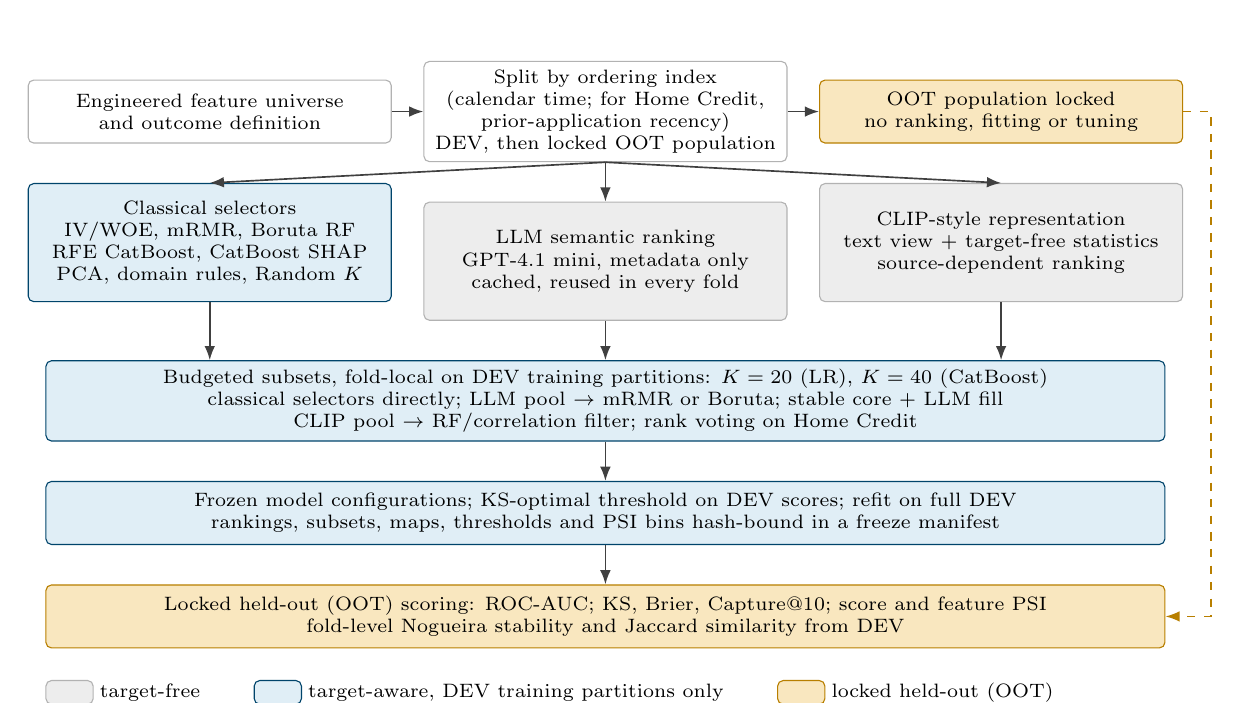
\begin{tikzpicture}[
    font=\scriptsize,
    box/.style={draw=gray!60, rounded corners=2pt, align=flush center, inner sep=3pt, minimum height=8mm, fill=white},
    tfree/.style={box, fill=gray!14},
    taware/.style={box, fill=cBlue!12, draw=cBlue!60!black},
    oot/.style={box, fill=cOrange!25, draw=cOrange!80!black},
    arr/.style={-{Latex[length=1.8mm]}, semithick, gray!50!black},
    darr/.style={-{Latex[length=1.8mm]}, semithick, dashed, cOrange!80!black},
    node distance=5mm and 4mm
]
\node[box, text width=44mm] (data) {Engineered feature universe\\and outcome definition};
\node[box, text width=44mm, right=of data] (split) {Split by ordering index\\(calendar time; for Home Credit,\\prior-application recency)\\DEV, then locked OOT population};
\node[oot, text width=44mm, right=of split] (ootheld) {OOT population locked\\no ranking, fitting or tuning};

\node[taware, text width=44mm, minimum height=15mm, below=of data] (classical) {Classical selectors\\IV/WOE, mRMR, Boruta RF\\RFE CatBoost, CatBoost SHAP\\PCA, domain rules, Random $\Kfeat$};
\node[tfree, text width=44mm, minimum height=15mm, below=of split] (llm) {LLM semantic ranking\\GPT-4.1 mini, metadata only\\cached, reused in every fold};
\node[tfree, text width=44mm, minimum height=15mm, below=of ootheld] (clip) {CLIP-style representation\\text view + target-free statistics\\source-dependent ranking};

\node[taware, text width=140mm, below=of llm] (subset) {Budgeted subsets, fold-local on DEV training partitions: $\Kfeat=20$ (LR), $\Kfeat=40$ (CatBoost)\\classical selectors directly; LLM pool $\rightarrow$ mRMR or Boruta; stable core + LLM fill\\CLIP pool $\rightarrow$ RF/correlation filter; rank voting on Home Credit};
\node[taware, text width=140mm, below=of subset] (model) {Frozen model configurations; KS-optimal threshold on DEV scores; refit on full DEV\\rankings, subsets, maps, thresholds and PSI bins hash-bound in a freeze manifest};
\node[oot, text width=140mm, below=of model] (eval) {Locked held-out (OOT) scoring: ROC-AUC; KS, Brier, Capture@10; score and feature PSI\\fold-level Nogueira stability and Jaccard similarity from DEV};

\draw[arr] (data) -- (split);
\draw[arr] (split) -- (ootheld);
\draw[arr] (split) -- (llm);
\draw[arr] (split.south) -- (classical.north);
\draw[arr] (split.south) -- (clip.north);
\draw[arr] (classical) -- (classical.south |- subset.north);
\draw[arr] (llm) -- (subset);
\draw[arr] (clip) -- (clip.south |- subset.north);
\draw[arr] (subset) -- (model);
\draw[arr] (model) -- (eval);
\draw[darr] (ootheld.east) -- ++(3.5mm,0) |- (eval.east);

\node[tfree, minimum height=3mm, minimum width=6mm, inner sep=0pt, anchor=north west] (l1) at ([yshift=-4mm]eval.south west) {};
\node[anchor=west, inner sep=2pt] (t1) at (l1.east) {target-free};
\node[taware, minimum height=3mm, minimum width=6mm, inner sep=0pt, anchor=west] (l2) at ([xshift=6mm]t1.east) {};
\node[anchor=west, inner sep=2pt] (t2) at (l2.east) {target-aware, DEV training partitions only};
\node[oot, minimum height=3mm, minimum width=6mm, inner sep=0pt, anchor=west] (l3) at ([xshift=6mm]t2.east) {};
\node[anchor=west, inner sep=2pt] at (l3.east) {locked held-out (OOT)};
\end{tikzpicture}
\caption{Research pipeline. Grey boxes are target-free stages that consume metadata and development statistics only; blue boxes are target-aware stages confined to DEV training partitions and refitted once on full DEV; orange boxes concern the locked held-out population (OOT), which enters only at the final scoring. The ordering index of the split is calendar time for LendingClub and Stability 2024 and prior-application recency for Home Credit.}
\label{fig:pipeline}
\end{figure*}

\subsection{Data Preprocessing}
\label{subsec:preprocessing}

Numeric variables are processed by replacing infinite values with missing values, imputing with the training-partition mean and standardising with training-partition statistics. Categorical variables receive an explicit missing token and are one-hot encoded; levels unseen in the training partition are ignored, and rare levels are dropped below a minimum frequency of 10 observations for Home Credit and Stability 2024 and 50 for LendingClub. The order of operations is fixed: eligibility screening and selection operate on \emph{original} features, one column per candidate, so a categorical variable is selected or rejected as a whole, and one-hot expansion is performed only after the subset has been selected, so that the budget $\Kfeat$ counts original variables. Principal-component selection is the one exception, since its retained quantities are components. Preprocessing maps are fitted on the training partition of each fold and, for the final model, on full DEV.

\subsection{Classical Feature-Selection Methods}
\label{subsec:classical_fs}

Table~\ref{tab:methods} lists the fourteen strategies and the full-feature reference. All target-aware selectors are fitted on the training partition of each fold with DEV labels only and refitted on full DEV before OOT scoring; unless stated otherwise, candidates are ranked by the method's own criterion and the top $\Kfeat$ original features are kept. \emph{IV/WOE} ranks by Eq.~\eqref{eq:iv} computed on the training partition with ten quantile bins \cite{siddiqi2006}, and the same statistic defines the eligibility interval used before the hybrids and the pre-screen of \emph{IV then Boruta}. \emph{mRMR} applies Eq.~\eqref{eq:mrmr} with mutual information estimated on the training partition \cite{peng2005,kraskov2004,ross2014}; its pool is the full eligible universe when it is used alone and the shortlist when it follows a semantic stage. Throughout the paper \emph{mRMR} denotes this mutual-information implementation; the random-forest/correlation rule used inside the contrastive branch is called the \emph{RF/correlation filter} (Section~\ref{subsec:clip_fs}) and was named legacy mRMR in the early versions of the study. \emph{Boruta RF} confirms features whose random-forest importance (500 trees of depth 6) exceeds the best shuffled shadow importance at $\alpha=0.05$ with two-step correction and keeps the top $\Kfeat$ confirmed features \cite{kursa2010,breiman2001}; when fewer than $\Kfeat$ features are confirmed, the subset consists of the confirmed features alone and is flagged as below budget, and tentative or rejected features are never added; \emph{RFE CatBoost} removes 20\% of the surviving features per step by the importance of an internal CatBoost ranker (500 iterations, depth 6, learning rate 0.05) until $\Kfeat$ remain \cite{guyon2002}; \emph{CatBoost SHAP} keeps the $\Kfeat$ features with the largest aggregate absolute SHAP contribution over a 10,000-row training sample \cite{lundberg2017}; \emph{PCA} retains the leading components and is reported as a transformation baseline \cite{jolliffe2016}. \emph{Domain rules} is a deterministic credit-domain scorer that reads no data and calls no model: 42 named-variable rules, family and string-pattern rules for bureau, instalment, credit-card and previous-application aggregates, 15 property-attribute rules and nine semantic-group fallbacks assign each feature a priority, which aggregation suffixes and leakage status adjust, with deterministic tie ordering. Remaining implementation details are fixed in the public code repository.

\begin{table*}[htbp]
\centering
\footnotesize
\begin{threeparttable}
\caption{Feature-selection strategies evaluated. ``Labels'' states whether the stage that produces the final subset uses DEV outcomes. The full-feature model is a reference and is excluded from selector comparisons.}
\label{tab:methods}
\begin{tabular}{@{}llL{52mm}c@{}}
\toprule
Method & Family & Selection role & Labels \\
\midrule
Full features & Reference & No selection; context only & -- \\
Domain rules & Classical & Eligibility and policy filters from credit-domain definitions & no \\
Random $\Kfeat$ & Baseline & Uniformly random subset of size $\Kfeat$; the floor for every selector & no \\
PCA & Classical & Leading components of the standardised candidates (components, not original features) & no \\
IV/WOE & Classical & Ranking by information value, Eq.~\eqref{eq:iv} & yes \\
mRMR & Classical & Mutual-information relevance against mutual-information redundancy, Eq.~\eqref{eq:mrmr} & yes \\
Boruta RF & Classical & All-relevant random-forest wrapper with shadow-feature comparison & yes \\
IV then Boruta & Classical hybrid & IV eligibility screen followed by Boruta confirmation & yes \\
RFE CatBoost & Model wrapper & Recursive elimination driven by CatBoost importance & yes \\
CatBoost SHAP & Embedded & Ranking by aggregated absolute SHAP contribution & yes \\
Pure LLM & LLM-assisted & Top-$\Kfeat$ names of the cached semantic ranking & no \\
LLM then mRMR & LLM hybrid & Semantic pool of 60 (LR) or 100 (CatBoost), then mRMR & yes \\
LLM then Boruta & LLM hybrid & Semantic pool, then Boruta confirmation & yes \\
Stable core + LLM fill & LLM hybrid & Bootstrap-stable RF/correlation core completed from the LLM ranking & yes \\
CLIP-ranked & Representation & Target-free contrastive ranking, then RF/correlation filter & yes \\
\bottomrule
\end{tabular}
\end{threeparttable}
\end{table*}

\subsection{Pure LLM Selection}
\label{subsec:llm_fs}

The language model is GPT-4.1 mini \cite{openai2025gpt41}, snapshot \path{gpt-4.1-mini-2025-04-14}, called through the Chat Completions interface with temperature 0 and a JSON response format; it never receives rows, outcomes, validation statistics or OOT information. Two information contracts are used, and the difference is deliberate. Under the \emph{training-statistics protocol} of Home Credit and LendingClub (prompt \texttt{stability\_expert\_v3}) the model receives the eligible feature names and descriptions together with training-only summaries (missingness, numeric moments and quantiles, categorical cardinality) and returns a ranked list of at most 100 known features; unknown names are rejected, duplicates removed, a short list is completed from the candidate order, and a failure after three retries falls back to a documented legacy ranking. Under the \emph{definition-only protocol} of Stability 2024 (prompt \texttt{stability\_expert\_v5}, strict JSON schema) the model receives the approved definition of each variable with its source table, origin, aggregation depth, data type, logical type and description hash, but no statistic computed on any row, and returns exactly 100 distinct known features under strict validation with up to three attempts and no fallback; the Stability ranking was accepted at the second attempt, after the first response contained one unknown name. Both prompt templates are reproduced in \ref{app:prompts}. The \emph{pure LLM} selector retains the top $\Kfeat$ names. The ranking is computed once per dataset and cached, so every fold, both backbones and the full-DEV refit use the same ordering; the cached ranking, rather than a fresh call, is the reproducible artefact, because a fixed model identifier and zero temperature do not guarantee identical outputs across independent calls.

\subsection{Hybrid Selection Methods}
\label{subsec:hybrid_fs}

Three hybrids combine the cached semantic ranking with target-aware refinement. \emph{LLM then mRMR} takes the top 60 (logistic regression) or top 100 (CatBoost) features of the ranking as the pool and applies mutual-information mRMR on the fold training partition to reach $\Kfeat$: the semantic stage is intended to remove variables an analyst would consider implausible or redundant in meaning and the statistical stage variables redundant in the data, although the semantic stage can also remove variables that a full-pool statistical selector would have used (Section~\ref{subsec:voting_results}). \emph{LLM then Boruta} applies Boruta confirmation to the same pool and truncates to the budget. \emph{Stable core + LLM fill} draws five bootstrap resamples of the fold training partition (80\% with replacement, seeds 42 to 46), runs the RF/correlation filter on each, keeps as the stable core the features selected in at least four of the five resamples, ordered by selection frequency and mean rank, and completes the subset from the LLM ranking in rank order without padding from unranked features, preserving the reproducibility of the core while letting semantically prioritised variables fill the remaining budget. None of these pipelines is target-free as a whole, and the fold-to-fold stability of a hybrid subset depends on both the fixed semantic ranking and the fitted target-aware stage.

\subsection{CLIP-Based Representation and Selection}
\label{subsec:clip_fs}

\begin{sloppypar}
Each feature is represented by two views: a text view that encodes the name and description (\texttt{feature\_\allowbreak text\_\allowbreak v1}) with the frozen \texttt{all-\allowbreak MiniLM-\allowbreak L6-\allowbreak v2} sentence encoder into a 384-dimensional $L_2$-normalised embedding \cite{wang2020minilm,reimers2019}, and a statistical view of 13 target-free descriptors (\texttt{compact\_\allowbreak target\_\allowbreak free\_\allowbreak v2}) computed on DEV feature values only. Two projection heads map the views into a shared space and are trained contrastively so that the two views of the same feature are aligned and the views of different features are separated \cite{radford2021,oord2018}; the pairing policy \texttt{identity\_\allowbreak equivalence\_\allowbreak v2} masks only verified identity-equivalent pairs from the negative set. Five representations are trained with seeds 11, 22, 33, 44 and 55; for each seed the checkpoint with minimum source-validation loss is kept after retrieval diagnostics on 395 held-out validation feature pairs (mean reciprocal rank, Recall@1/5/10, cosine margin between positive pairs and allowed negatives) and collapse diagnostics, and the five spaces are aligned to the seed-11 space by orthogonal Procrustes rotation \cite{schonemann1966}, averaged and re-normalised. The consensus space defines a source anchor against which features are scored and ranked.
\end{sloppypar}

Three source representations rank the same 1,959 Stability 2024 predictors: the native representation trained on Stability DEV statistics, and the Home Credit and LendingClub representations applied frozen, each with its own descriptor transform, projectors and anchor, without refitting and without Stability labels; agreement is measured by Spearman correlation \cite{spearman1904} and by shared top-100 features. The contrastive ranking is a candidate prior, not a selector: logistic regression uses the top 60 ranked features and CatBoost the top 100, and a target-aware redundancy stage reduces the pool to $\Kfeat$. This stage is the \emph{RF/correlation filter}, a greedy relevance-to-redundancy rule in which relevance $R_j$ is the importance from a random forest of 128 trees fitted on the fold training partition, redundancy is the mean absolute Pearson correlation with the features already selected, and the score is
\begin{equation}
    \mathrm{score}(j\mid S)=\frac{R_j}{\max\{0.05,\ |S|^{-1}\sum_{k\in S}|\rho(X_j,X_k)|\}} ,
    \label{eq:legacy_mrmr}
\end{equation}
with a redundancy floor of 0.05. Because the representation is built from frozen full-DEV feature distributions and not recomputed inside each row fold, fold-level scores in this branch are diagnostic and the locked OOT evaluation is decisive. A pre-OOT validation recorded 29 of 29 leakage checks passing (no target values, OOT feature values, OOT labels, prior selector ranks, prior model outputs or LLM rankings consumed) and 287 of 287 declared SHA-256 checks on the frozen artefacts.

\subsection{Voting / Rank Aggregation}
\label{subsec:voting_fs}

The voting experiment asks whether the sequential order \emph{LLM then statistical refinement} discards information that a parallel combination would retain. It is run on Home Credit over the full universe of $d=529$ features. For a feature with rank $r$ in a source ranking (rank 1 best) the normalised rank is
\begin{equation}
    r^{\mathrm{norm}}=\frac{r-1}{d-1},
    \label{eq:normrank}
\end{equation}
so that the best feature maps to 0 and the worst to 1. The two-voter score averages the normalised LLM and contrastive ranks; the top $P\in\{100,200,300\}$ features form a pool that mutual-information mRMR reduces to $\Kfeat=20$ or $40$, with ties resolved by LLM rank, then contrastive rank, then feature name. A \emph{direct three-voter} variant averages the normalised LLM, contrastive and mRMR relevance ranks and selects the top $\Kfeat$ without refinement. The full-universe LLM ranking was generated from label-free metadata for all 529 features, the contrastive coverage was extended deterministically to 93 features lacking descriptors using the frozen representation and DEV-only descriptors, and the mRMR relevance ranking used DEV labels only. Averaging normalised ranks is a Borda-type rule \cite{dwork2001} in the tradition of ensemble feature selection \cite{saeys2008}.

\subsection{Development of the Protocol}
\label{subsec:protocol_development}

The protocol above is the final form of an evaluation developed through successive versions, and the final results supersede the earlier ones. Table~\ref{tab:stages} records the changes that mattered and their consequences. The DEV/OOT design of Home Credit and LendingClub was fixed from the outset, and the Stability 2024 cutoff was moved once, from 2020-02-26 to 2020-02-01, for the final evaluation (Section~\ref{subsec:dev_oot}); what changed otherwise was the comparator set, the semantic inputs of the LLM stage, the statistical selector used as the classical reference, the inference procedure, and the correctness of the reported values. Three changes moved the numbers. First, the comparator changed from a single mRMR baseline on two datasets to the per-case best classical selector drawn from the full selector set on three datasets, a stricter test for the LLM-assisted pipelines. Second, the semantic representation of the features supplied to the language model, the descriptions and lineage that the two information contracts formalise, was revised between the early versions and the final protocol, and this revision is the main reason the LLM-related scores of the final tables differ from those of the early versions. Third, the mutual-information mRMR of the final protocol replaced the RF/correlation filter of the early versions as the stand-alone statistical selector, which is why the Home Credit logistic-regression mRMR reference of the final tables (0.7699) differs from the earlier value (0.7457). Two inference changes altered what could be claimed rather than the estimates: five-fold rank tests, whose minimum attainable two-sided $p$-value with five non-zero pairs is 0.0625, gave way to paired inference on matched OOT observations, and the six headline comparisons were prespecified with confidence intervals and Holm correction. Finally, earlier report versions contained transcription and rounding errors that the final revision corrected. Earlier values are therefore superseded and are quoted only where the text says so.

\begin{table*}[htbp]
\centering
\footnotesize
\setlength{\tabcolsep}{5pt}
\begin{threeparttable}
\caption{Protocol versions preceding the final evaluation. Values quoted in the last column are superseded values, computed with earlier comparator sets, earlier semantic inputs and, in the earliest versions, the RF/correlation filter as the mRMR reference.}
\label{tab:stages}
\begin{tabular}{@{}L{27mm}L{\dimexpr(\textwidth-27mm-4\tabcolsep)/2\relax}L{\dimexpr(\textwidth-27mm-4\tabcolsep)/2\relax}@{}}
\toprule
Protocol version & Change to the methodology & Effect on the results, and why (superseded values) \\
\midrule
Home Credit comparison & 16 pipelines on 529 features; the LLM produces a top-100 pool refined by mRMR, Boruta or a stable-core rule; six LLM calls reused across pipelines. & Best OOT AUC from CatBoost with LLM then mRMR (0.772 against 0.769 for mRMR). A variant whose LLM shortlist was almost as small as the budget gave no gain, so the LLM was fixed as a broad first-pass screener rather than the final selector. \\
\addlinespace
Corrected contrastive representation & Identity-equivalence pairing policy; incremental evaluation of the representation after LLM screening; bidirectional transfer diagnostics with LendingClub as source. & OOT AUC changed by less than 0.002 while fold Jaccard rose by 0.32 to 0.50; the contrastive branch was assigned to reproducibility and portability rather than discrimination. \\
\addlinespace
Two-dataset canonical comparison & Home Credit and LendingClub, four selectors, 16 runs; five-fold exact Wilcoxon tests; type-aware feature PSI repaired for 480 selected-feature occurrences; usage and cost accounting. & No fold test could reach $p<0.05$ (minimum attainable 0.0625), so fold tests were abandoned as underpowered; pure LLM had lower feature drift in three of four cells; direct API cost bounded at USD 0.171 to 0.413. \\
\addlinespace
Matched OOT inference and voting & Paired DeLong tests and 2,000-resample paired bootstrap on matched observation identifiers, Holm correction within families; eight voting variants added. & 11 of 12 canonical differences became significant, with dataset-dependent signs; voting exceeded sequential screening in 5 of 8 variants and full-pool mRMR in none. \\
\addlinespace
Three-dataset evaluation & Stability 2024 added (OOT cutoff 2020-02-26); fourteen selectors and a full-feature reference; revised semantic representation of the features supplied to the LLM, with the definition-only contract for Stability 2024; three-source contrastive extension; per-case best classical comparator. & LLM-assisted led five of six AUC cases at the point-estimate level; CLIP subset reproducibility and source-dependent transfer established; the stricter comparator lowered the apparent LLM advantage relative to the two-dataset comparison, while the revised semantic inputs raised the LLM-related scores. \\
\addlinespace
Final revised evaluation (this paper) & Stability 2024 OOT cutoff moved from 2020-02-26 to 2020-02-01 to balance event rates (3.16\% DEV, 3.09\% OOT); six prespecified paired comparisons with confidence intervals and Holm correction; exact AUC precision; mutual-information mRMR distinguished from the RF/correlation filter; transcription and rounding errors of earlier versions corrected. & Results of Section~\ref{sec:results}; the contrastive extension and the two Stability full-feature references were not re-run and remain on the 2020-02-26 cohort, so they are compared with the headline selectors descriptively only. \\
\bottomrule
\end{tabular}
\end{threeparttable}
\end{table*}

% ============================================================
% 5. EXPERIMENTAL SETUP
% ============================================================

\section{Experimental Setup}
\label{sec:experimental_setup}

\subsection{Datasets}
\label{subsec:datasets}

Three public credit datasets released through Kaggle are used (Table~\ref{tab:datasets}). \emph{Home Credit} is the Home Credit Default Risk data \cite{homecredit2018}: the unit is a loan application, the event is the provider's binary target (payment difficulties), and the universe contains 529 original features derived from the application record and the auxiliary tables, of which 391 pass eligibility screening. \emph{LendingClub v2} is the LendingClub loan book \cite{lendingclub_kaggle}: only resolved 36- and 60-month loans through the 2019-05-01 snapshot are retained, with charged-off or defaulted loans as events and fully paid loans as non-events, and the universe has 675 original features, of which 161 pass screening. The ordering index differs between the two. For Home Credit it is \texttt{DAYS\_DECISION}, the number of days between the applicant's most recent previous application and the current application, so the split is a recency-based covariate-shift holdout rather than a calendar-time split of the current applications: DEV holds applicants whose most recent previous application is 241 to 600 days old and OOT those with a more recent one, and applications without a previous application within the 600-day window are excluded, which limits the population to which the Home Credit results apply. For LendingClub the index is the number of days from the issue month to the last finalised issue month, 2018-12-01, so its OOT window is later in calendar time. \emph{Stability 2024} is the Home Credit Credit Risk Model Stability data \cite{homecredit2024}: the unit is a credit decision dated by \texttt{date\_decision}, the event is the provider's default target, and 1,959 engineered features were constructed from the 434 approved raw predictors, of which the 1,068 with at most 90\% missing values on the earliest training fold form the LLM candidate set. Home Credit and Stability 2024 share institutional lineage, whereas LendingClub is a distinct peer-to-peer platform, which matters for the transfer experiments.

\begin{table*}[htbp]
\centering
\footnotesize
\begin{threeparttable}
\caption{Datasets, held-out partitions and feature universes. OOT labels the locked held-out population of each dataset. Home Credit windows are days of the most recent previous-application decision relative to the current application, a recency-based covariate-shift holdout rather than a calendar-time split; LendingClub windows are days from the issue month to 2018-12-01; Stability 2024 windows are calendar dates of \texttt{date\_decision}. Validation blocks are the held-out sizes of the five expanding-window folds.}
\label{tab:datasets}
\begin{tabular}{@{}lL{29mm}L{31mm}L{31mm}@{}}
\toprule
 & Home Credit & LendingClub v2 & Stability 2024 \\
\midrule
Observation unit & Loan application & Issued loan & Credit decision \\
Event definition & Payment difficulties (provider target) & Charged off or default; resolved loans only & Default (provider target) \\
DEV window & day $-600$ to $-241$ & day $-1795$ to $-1096$ & 2019-01-01 to 2020-01-31 \\
DEV $N$ & 99,092 & 598,649 & 1,157,512 \\
DEV event rate & 7.93\% & 19.54\% & 3.16\% \\
OOT window & day $-240$ to $-1$ & day $-1065$ to $-730$ & 2020-02-01 to 2020-10-05 \\
OOT $N$ & 120,053 & 293,105 & 369,147 \\
OOT event rate & 8.90\% & 23.29\% & 3.09\% \\
Validation blocks & 16,720; 16,638; 16,401; 16,625; 16,263 & 114,267; 86,170; 126,995; 99,837; 71,911 & \textbf{[recompute: five validation blocks of the 2020-01-31 DEV]} \\ % TODO: the previous values (204,567; 203,798; 205,980; 201,466; 202,820) belong to the 2020-02-26 cohort
Feature universe & 529 original features & 675 original features & 1,959 engineered features \\
LLM candidate set & 391 eligible & 161 eligible & 1,068 of 1,959 ($\le$90\% missing) \\
\bottomrule
\end{tabular}
\begin{tablenotes}\footnotesize
\item The Stability 2024 column describes the cohort of the headline evaluation (cutoff 2020-02-01). The contrastive extension (Table~\ref{tab:clip_cells}) and the two Stability full-feature reference models (Table~\ref{tab:primary_results}) use the earlier cohort: DEV 2019-01-01 to 2020-02-25 (1,221,743 decisions, 3.24\%), OOT 2020-02-26 to 2020-10-05 (304,916 decisions, 8,349 events, 2.74\%).
\end{tablenotes}
\end{threeparttable}
\end{table*}

\subsection{Held-Out DEV/OOT Design}
\label{subsec:dev_oot}

Each dataset is partitioned along its ordering index into a development population (DEV) and a locked held-out population (OOT). For LendingClub and Stability 2024 the index is calendar time and OOT is later than DEV, which addresses whether a selected subset and a fitted model still rank risk correctly on loans issued or decisions taken after development; random splits would mask both population drift and the optimism of subsets tuned on the same period \cite{bergmeir2012,gama2014}. For Home Credit the index is prior-application recency, so OOT is a recency-based covariate-shift holdout of applicants with a more recent previous application, not a set of later applications. Within DEV, five expanding-window folds are formed along the same index, each training partition consisting of the lowest-index observations and the validation partition of a later block (sizes in Table~\ref{tab:datasets}) separated by a gap of one index group, one index day for Home Credit and LendingClub and one decision date for Stability 2024; for Home Credit these folds are ordered by recency rather than by application date. Every component is fitted on the training partition, applied to the validation partition without refitting, and refitted once on full DEV after development.

For Stability 2024 the OOT cutoff of the headline evaluation is 2020-02-01: DEV comprises the 1,157,512 decisions dated 2019-01-01 to 2020-01-31 (event rate 3.16\%) and OOT the 369,147 decisions dated 2020-02-01 to 2020-10-05 (3.09\%), 24.2\% of the 1,526,659 decisions. During protocol development the cutoff was 2020-02-26 (DEV 1,221,743 decisions at 3.24\%; OOT 304,916 decisions with 8,349 events, 2.74\%). It was moved 25 days earlier for the final evaluation, after the earlier run had been scored, because the later tail compared the development population with a materially lower-risk OOT population. The contrastive extension of Section~\ref{subsec:clip_results} and the two Stability full-feature reference models of Table~\ref{tab:primary_results} were not re-run and are reported on the 2020-02-26 cohort; they are not scored on the same OOT population as the headline comparisons and are compared with them descriptively only. The LendingClub OOT window ends at day $-730$ (loans issued through 2016-12), and only loans resolved by the 2019-05-01 snapshot are evaluated. This restriction can preferentially retain early defaults and early repayments when other loans of the same cohort remain unresolved, and follow-up duration differs across issue cohorts and between 36- and 60-month terms, so population composition and the reported DEV--OOT event-rate difference (Table~\ref{tab:datasets}) should be read with this selection in mind. Before the OOT population is opened, the eligible universe, the cached LLM rankings, the contrastive representations and rankings, every selected subset, the preprocessing maps, the model configurations and fitted models, the operating thresholds and the DEV score bins used as PSI references are frozen; OOT outcomes are used only to compute the reported metrics, the one exception being the Stability 2024 event rate that informed the cutoff described above.

\subsection{Predictive Models}
\label{subsec:models}

Two backbones are used in every dataset--selector case, spanning a linear scorecard-style model and a non-linear boosted model \cite{lessmann2015,gunnarsson2021}, with configurations fixed and identical across selectors. The logistic regression uses the \texttt{liblinear} solver of scikit-learn \cite{pedregosa2011} with an L2 penalty and $C=1$, at most 1,000 iterations, balanced class weights and random seed 42. CatBoost \cite{prokhorenkova2018} uses depth 10, learning rate 0.01, L2 leaf regularisation 95, minimum 290 observations per leaf, a feature-sampling rate (\texttt{rsm}) of 0.90, random strength 0.125, depthwise growth, Bernoulli bootstrap with subsample 0.55, the Logloss objective with AUC evaluation, balanced class weights, seed 42, four threads and a fixed 1,500 iterations without early stopping, so that no validation information enters the fitted model. Balanced class weights are used because event rates range from about 3\% to 23\%.

\subsection{Feature Budgets}
\label{subsec:feature_budgets}

The budgets are $\Kfeat=20$ original features for logistic regression and $\Kfeat=40$ for CatBoost. They were determined in DEV-only experimentation and frozen before OOT evaluation: larger linear subsets added redundancy without a competitive improvement in development discrimination, whereas CatBoost continued to benefit from a larger subset and was less sensitive to redundant predictors. The budgets are model-specific rather than dataset-specific, so selectors within a backbone are compared at equal subset size, whereas comparisons between backbones differ in both model class and budget.

\subsection{Evaluation Metrics}
\label{subsec:metrics}

Let $y_i\in\{0,1\}$ be the event label of OOT observation $i$, $p_i$ its predicted event probability, $N_+$ and $N_-$ the numbers of events and non-events, and $N=N_++N_-$.

\paragraph{ROC-AUC}
The area under the receiver operating characteristic curve is the probability that a randomly chosen event scores higher than a randomly chosen non-event, with half credit for ties \cite{hanley1982},
\begin{equation}
    \AUC=\frac{1}{N_+N_-}\sum_{i:\,y_i=1}\sum_{j:\,y_j=0}\big[\mathbf{1}(p_i>p_j)+\tfrac12\mathbf{1}(p_i=p_j)\big].
    \label{eq:roc_auc}
\end{equation}
Higher is better. ROC-AUC is threshold-free and is the sole headline metric; the Gini coefficient $2\,\AUC-1$ adds no information.

\paragraph{KS}
The Kolmogorov--Smirnov statistic is the maximum vertical separation between the cumulative score distributions of events and non-events,
\begin{equation}
    \KS=\max_{t}\,\big[\TPR(t)-\FPR(t)\big],
    \label{eq:ks}
\end{equation}
which equals the maximum Youden index over thresholds \cite{youden1950}; higher is better. The operating threshold of each model is the DEV training-score threshold at which this separation is maximal (the first maximum when ties occur), frozen and applied unchanged to OOT; the paper reports KS as the maximum OOT separation rather than the separation at the frozen threshold.

\paragraph{Brier score}
The Brier score is the mean squared error of the predicted probabilities \cite{brier1950},
\begin{equation}
    \mathrm{Brier}=\frac{1}{N}\sum_{i=1}^{N}(y_i-p_i)^2 ,
    \label{eq:brier}
\end{equation}
lower is better. It measures the overall squared error of the predicted probabilities, which combines calibration and resolution, rather than ranking; a constant prediction equal to the event rate $\pi$ attains $\pi(1-\pi)$, and log loss, $-N^{-1}\sum_i[y_i\ln p_i+(1-y_i)\ln(1-p_i)]$, is a supporting diagnostic. Because both backbones use balanced class weights and no recalibration (Section~\ref{subsec:models}), their outputs are not population event probabilities, so Brier values compare selectors within a dataset and do not indicate deployment-ready calibration.

\paragraph{Capture@10 and Lift@10}
Let $T$ be the set of observations in the highest-scored decile, a fraction $q=|T|/N\approx0.10$ of the population. Capture@10 is the share of all events found in that decile and Lift@10 the ratio of the decile event rate to the portfolio event rate,
\begin{equation}
\begin{aligned}
    \mathrm{Capture@10}&=\frac{\sum_{i\in T}y_i}{\sum_{i}y_i},\\
    \mathrm{Lift@10}&=\frac{|T|^{-1}\sum_{i\in T}y_i}{N^{-1}\sum_{i}y_i}=\frac{\mathrm{Capture@10}}{q};
\end{aligned}
    \label{eq:capture10}
\end{equation}
higher is better, and Lift equals ten times Capture only when the decile is exact.

\paragraph{PSI}
The population stability index compares a reference distribution with a later distribution over frozen states $b$,
\begin{equation}
    \PSI=\sum_{b}\big(o_b-r_b\big)\ln\frac{o_b}{r_b},
    \label{eq:psi}
\end{equation}
where $r_b$ and $o_b$ are the reference (DEV) and OOT proportions in state $b$ \cite{siddiqi2006,yurdakul2020}; lower indicates less shift. For \emph{score PSI} the states are ten quantile bins of the DEV out-of-fold scores, with duplicate edges collapsed and proportions floored at $10^{-6}$; the reference distribution is thus formed from out-of-fold predictions of the five fold models, whereas the OOT scores come from the model refitted on full DEV, so score PSI can reflect differences between scoring models as well as population change. For \emph{feature PSI} the states are type-aware: DEV quantile bins plus a missing state for continuous variables, explicit 0/1/missing/unexpected states for binary and one-hot variables, exact DEV levels for discrete variables, and DEV categories plus missing and unseen states for source categoricals. Bins and states are learned on DEV, frozen and applied unchanged to OOT; mean, median and maximum feature PSI over the selected subset summarise drift within the chosen inputs. A feature PSI of zero means that no distribution difference was detected under the implemented states, binning and numerical precision, not that the underlying distributions are identical. The conventional references of 0.10 and 0.25 are descriptive monitoring thresholds, not critical values \cite{yurdakul2020}.

\paragraph{Nogueira stability}
Let $Z_{fj}\in\{0,1\}$ indicate whether feature $j$ of a candidate universe of size $d$ is selected in development fold $f=1,\dots,B$ with $B=5$. With $\hat p_j=B^{-1}\sum_f Z_{fj}$, $s_j^2=\frac{B}{B-1}\hat p_j(1-\hat p_j)$ and $\bar k=\sum_j \hat p_j$, the Nogueira estimator is \cite{nogueira2018}
\begin{equation}
    \hat\Phi=1-\frac{d^{-1}\sum_{j=1}^{d}s_j^2}{(\bar k/d)\,(1-\bar k/d)} .
    \label{eq:nogueira}
\end{equation}
It equals 1 when the same subset is selected in every fold, is chance-corrected so that random selection gives values near 0, and can be negative. The universe $d$ is the pool from which the fold-local selector chose: the eligible universe for classical selectors and the top-60 or top-100 pool for the contrastive branch. A ranking reused unchanged across folds has trivial perfect stability, so $\hat\Phi$ is reported only for selectors refitted in each fold.

\paragraph{Jaccard similarity}
For fold subsets $S_a$ and $S_b$ the Jaccard similarity is $J(S_a,S_b)=|S_a\cap S_b|/|S_a\cup S_b|$ \cite{jaccard1901}, and mean pairwise Jaccard averages $J$ over the $B(B-1)/2=10$ unordered pairs of folds; higher indicates more reproducible selection. Unlike Eq.~\eqref{eq:nogueira} it is not chance-corrected and does not depend on $d$, so the two statistics are reported together.

\subsection{Statistical Inference}
\label{subsec:inference}

Six paired comparisons were prespecified, one for each combination of dataset and backbone: the best LLM-assisted selector against the best classical selector of the case; the method matrices, feature budgets, comparison graph and inference families were fixed before OOT scoring. The two pipelines are scored on identical OOT observations paired by observation identifier (\texttt{SK\_\allowbreak ID\_\allowbreak CURR} for Home Credit, a stable identifier derived from the processed source row for LendingClub, the decision identifier for Stability 2024). The null hypothesis is a zero paired OOT ROC-AUC difference; the two-sided paired DeLong test \cite{delong1988} is used, 95\% confidence intervals are obtained from 2,000 target-stratified paired bootstrap resamples that draw the same observation indices for both pipelines \cite{efron1993} with seed 20260721, and Holm's step-down procedure \cite{holm1979} controls the family-wise error rate across the six comparisons at $\alpha=0.05$. Positive differences favour the LLM-assisted selector. Comparisons against the full-feature reference and among secondary metrics are descriptive point estimates. The Home Credit voting experiment used the same paired procedure with Holm correction within its own family of 24 tests, in which each of the eight voting variants is compared with three comparators: the sequential pipeline LLM then mRMR, full-pool mRMR, and LLM then CLIP then mRMR. Because large OOT samples make small differences detectable, effect sizes and intervals are always reported with the $p$-values \cite{demsar2006}.

\subsection{Leakage and Reproducibility Controls}
\label{subsec:leakage_controls}

OOT rows are excluded from eligibility screening, feature selection, ranking construction, representation training, hyperparameter choice, threshold selection and PSI reference construction; all target-aware components are fitted fold-locally inside DEV and refitted once on full DEV. The language model receives no validation or OOT statistics under either contract, and the contrastive representation consumes no target values, OOT feature values, prior selector ranks, prior model outputs or LLM rankings. Cached rankings, contrastive checkpoints, selected subsets, preprocessing maps, model settings, thresholds and PSI references are frozen and hash-bound before OOT scoring. Randomness is controlled by fixed seeds (42 for both classifiers and the selectors, 42 to 46 for the stable-core resamples, the five declared seeds of the representation, 20260721 for the inference bootstrap), and the LLM is called with temperature 0 and a fixed snapshot with its rankings cached. Experiments ran in Python 3.13.5 with scikit-learn 1.8.0, CatBoost 1.2.10 and Boruta 0.4.3 on a laptop with an Intel Core i7-13620H processor (10 cores) and 40~GiB of memory, on the CPU with four estimator threads, one experiment and one fold at a time. Datasets are public, and code, configuration files and experiment artefacts are available in the repository listed in the Data availability statement.

% ============================================================
% 6. RESULTS
% ============================================================

\section{Results}
\label{sec:results}

\subsection{Primary OOT Comparison}
\label{subsec:primary_results}

Table~\ref{tab:primary_results} and Figure~\ref{fig:primary} report the six prespecified comparisons that answer RQ1. LLM-assisted selection has a significantly higher held-out ROC-AUC than the best classical selector in five of the six dataset--backbone cases, and the classical selector is significantly higher in the sixth; all six Holm-adjusted $p$-values are below 0.05. Across the six cases the leading LLM-assisted method is pure LLM in four (Home Credit CatBoost, LendingClub v2 LR, Stability 2024 LR and Stability 2024 CatBoost), LLM then mRMR in one (LendingClub v2 CatBoost) and stable core plus LLM fill in the remaining case, Home Credit LR, where the classical selector leads. The pattern is dataset- and model-specific. LendingClub v2 and Stability 2024 favour LLM-assisted selection under both backbones, with pure LLM screening the best LLM-assisted selector in three of those four cases and LLM then mRMR in the fourth, and with differences of $+0.028$ to $+0.051$. Home Credit is mixed: with CatBoost, pure LLM exceeds the RFE CatBoost wrapper by $+0.012$, whereas with logistic regression mutual-information mRMR exceeds the best LLM-assisted pipeline, stable core plus LLM fill, by $0.021$. The best classical comparator changes identity across cases (mRMR, RFE CatBoost or IV then Boruta), so a single classical baseline would have misrepresented the strength of classical selection; and because the classical arm selects the best of nine selectors while the LLM-assisted arm selects the best of four, the comparator is the stronger of the two references and the five LLM-assisted wins are conservative in this respect. The largest gain occurs on LendingClub with CatBoost, the dataset whose eligible universe is the smallest after screening (161 of 675 features) and whose OOT event rate is the highest. Against models fitted on the full eligible universe (column ``Full''), the best compact subset of 20 or 40 original features has the higher OOT AUC in three of the four cases whose reference was fitted on the same cohort, by $+0.007$ (Home Credit, CatBoost) to $+0.048$ (LendingClub v2, CatBoost); the exception is again Home Credit logistic regression, where the full-feature model is $0.0016$ above the mRMR subset. The two Stability 2024 references come from the earlier 2020-02-26 cohort (Section~\ref{subsec:dev_oot}) and lie $0.061$ and $0.068$ below the compact subsets, but that comparison crosses cohorts. These are point estimates: no equivalence or non-inferiority test was performed, and all full-feature differences are descriptive, since no paired interval was computed against the reference. Table~\ref{tab:llm_pipelines} reports the held-out AUC of all four LLM-assisted pipelines on Home Credit and LendingClub v2. Pure LLM screening is within 0.009 of the best LLM-assisted pipeline in three of the four cases, LLM then mRMR leads it by 0.057 on LendingClub v2 CatBoost, and LLM then Boruta has the lowest AUC among the LLM-assisted pipelines in every case. On Stability 2024, stable core plus LLM fill attains 0.6815 with logistic regression and 0.8146 with CatBoost, against 0.8344 and 0.8784 for pure LLM screening.

\begin{table*}[htbp]
\centering
\scriptsize
\setlength{\tabcolsep}{3pt}
\begin{threeparttable}
\caption{Primary locked held-out (OOT) comparison. In each dataset--backbone case the best LLM-assisted and the best classical selector are compared on identical OOT observations. AUC is shown to four decimals; $\Delta$AUC, LLM-assisted minus classical, and its paired 95\% confidence interval are computed at full precision, with the Holm-adjusted $p$-value (family of six tests). ``Full'' is the OOT AUC of the full-feature reference model, shown for context only.}
\label{tab:primary_results}
\begin{tabular}{@{}L{21mm}L{25mm}L{22mm}rL{36mm}r@{}}
\toprule
Case & Best LLM-assisted (AUC) & Best classical (AUC) & Full & $\Delta$AUC [95\% CI] & Holm $p$ \\
\midrule
Home Credit, LR & Stable core + LLM fill\newline (0.7489) & mRMR\newline (0.7699) & 0.7715 & $-0.021033$\newline $[-0.031907,\,-0.010159]$ & $3.0\times10^{-4}$ \\
\addlinespace
Home Credit, CatBoost & Pure LLM\newline (0.7935) & RFE CatBoost\newline (0.7814) & 0.7860 & $+0.012024$\newline $[+0.001532,\,+0.022516]$ & 0.0247 \\
\addlinespace
LendingClub v2, LR & Pure LLM\newline (0.7402) & IV then Boruta\newline (0.7098) & 0.7109 & $+0.030431$\newline $[+0.025766,\,+0.035096]$ & $1.0\times10^{-36}$ \\
\addlinespace
LendingClub v2, CatBoost & LLM then mRMR\newline (0.7707) & IV then Boruta\newline (0.7201) & 0.7230 & $+0.050517$\newline $[+0.045959,\,+0.055075]$ & $7.2\times10^{-104}$ \\
\addlinespace
Stability 2024, LR & Pure LLM\newline (0.8344) & IV then Boruta\newline (0.8030) & 0.7734\tnote{a} & $+0.031444$\newline $[+0.020319,\,+0.042569]$ & $1.1\times10^{-7}$ \\
\addlinespace
Stability 2024, CatBoost & Pure LLM\newline (0.8784) & RFE CatBoost\newline (0.8500) & 0.8105\tnote{a} & $+0.028431$\newline $[+0.018409,\,+0.038453]$ & $1.1\times10^{-7}$ \\
\bottomrule
\end{tabular}
\begin{tablenotes}\scriptsize
\item[a] Reference values from the earlier complete run on the 2020-02-26 cohort (Section~\ref{subsec:dev_oot}); these two models were not refitted on the final split, so their differences from the selector AUCs are cross-cohort and descriptive.
\end{tablenotes}
\end{threeparttable}
\end{table*}

\begin{table}[htbp]
\centering
\footnotesize
\caption{Held-out (OOT) ROC-AUC of the four LLM-assisted pipelines on Home Credit and LendingClub v2 under both backbones ($\Kfeat=20$ for logistic regression, $\Kfeat=40$ for CatBoost). The largest value in each column is the LLM-assisted entry of Table~\ref{tab:primary_results}.}
\label{tab:llm_pipelines}
\setlength{\tabcolsep}{4pt}
\begin{tabular}{@{}lrrrr@{}}
\toprule
 & \multicolumn{2}{c}{Home Credit} & \multicolumn{2}{c}{LendingClub v2} \\
\cmidrule(lr){2-3}\cmidrule(l){4-5}
Pipeline & LR & CatBoost & LR & CatBoost \\
\midrule
Pure LLM & 0.7400 & 0.7935 & 0.7402 & 0.7137 \\
LLM then mRMR & 0.7381 & 0.7630 & 0.6907 & 0.7707 \\
LLM then Boruta & 0.6488 & 0.7592 & 0.6479 & 0.6850 \\
Stable core + LLM fill & 0.7489 & 0.7683 & 0.6840 & 0.7028 \\
\bottomrule
\end{tabular}
\end{table}

\begin{figure*}[htbp]
\centering
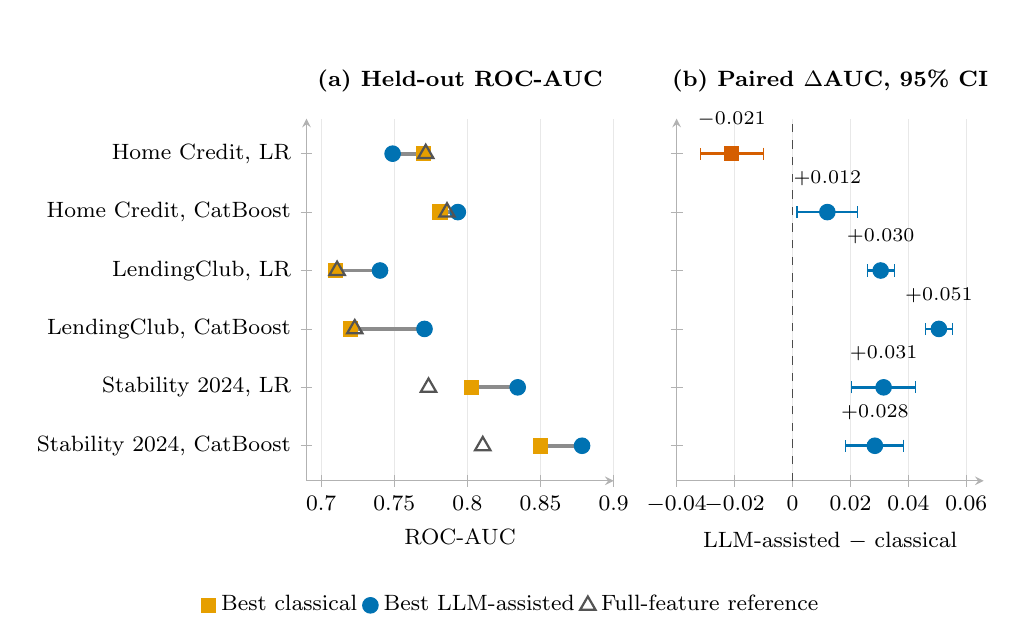
\begin{tikzpicture}
\begin{groupplot}[
    paper,
    group style={group size=2 by 1, horizontal sep=8mm, y descriptions at=edge left},
    scale only axis, width=3.9cm, height=4.6cm,
    ymin=0.4, ymax=6.6, ytick={1,2,3,4,5,6},
    yticklabels={{Stability 2024, CatBoost},{Stability 2024, LR},{LendingClub, CatBoost},{LendingClub, LR},{Home Credit, CatBoost},{Home Credit, LR}},
    xmajorgrids, axis lines=left, clip=false,
    xticklabel style={/pgf/number format/fixed, /pgf/number format/precision=2},
]
\nextgroupplot[title={(a) Held-out ROC-AUC}, xlabel={ROC-AUC}, xmin=0.69, xmax=0.90, xtick={0.70,0.75,0.80,0.85,0.90},
    legend to name=primlegend, legend columns=3]
\addplot[cGrey, line width=1.4pt, forget plot] coordinates {(0.849969,1) (0.878400,1)};
\addplot[cGrey, line width=1.4pt, forget plot] coordinates {(0.802956,2) (0.834400,2)};
\addplot[cGrey, line width=1.4pt, forget plot] coordinates {(0.720147,3) (0.770664,3)};
\addplot[cGrey, line width=1.4pt, forget plot] coordinates {(0.709803,4) (0.740234,4)};
\addplot[cGrey, line width=1.4pt, forget plot] coordinates {(0.781426,5) (0.793450,5)};
\addplot[cGrey, line width=1.4pt, forget plot] coordinates {(0.769890,6) (0.748857,6)};
\addplot[only marks, mark=square*, mark size=2.6pt, cOrange]
    coordinates {(0.849969,1) (0.802956,2) (0.720147,3) (0.709803,4) (0.781426,5) (0.769890,6)};
\addlegendentry{Best classical}
\addplot[only marks, mark=*, mark size=2.8pt, cBlue]
    coordinates {(0.878400,1) (0.834400,2) (0.770664,3) (0.740234,4) (0.793450,5) (0.748857,6)};
\addlegendentry{Best LLM-assisted}
\addplot[only marks, mark=triangle, mark size=3.2pt, thick, cGrey!60!black]
    coordinates {(0.8105,1) (0.7734,2) (0.722973,3) (0.710887,4) (0.786032,5) (0.771496,6)};
\addlegendentry{Full-feature reference}
\nextgroupplot[title={(b) Paired $\Delta$AUC, 95\% CI}, xlabel={LLM-assisted $-$ classical}, xmin=-0.04, xmax=0.066, xtick={-0.04,-0.02,0,0.02,0.04,0.06}]
\draw[gray!60!black, dashed] (axis cs:0,0.4) -- (axis cs:0,6.6);
\addplot[only marks, mark=*, mark size=2.8pt, cBlue,
    error bars/.cd, x dir=both, x explicit,
    error bar style={line width=1pt, cBlue},
    error mark options={rotate=90, mark size=2.2pt, cBlue}]
    coordinates {
        (0.028431,1) +- (0.010022,0)
        (0.031444,2) +- (0.011125,0)
        (0.050517,3) +- (0.004558,0)
        (0.030431,4) +- (0.004665,0)
        (0.012024,5) +- (0.010492,0)
    };
\addplot[only marks, mark=square*, mark size=2.6pt, cRed,
    error bars/.cd, x dir=both, x explicit,
    error bar style={line width=1pt, cRed},
    error mark options={rotate=90, mark size=2.2pt, cRed}]
    coordinates { (-0.021033,6) +- (0.010874,0) };
\node[font=\scriptsize, above=6pt] at (axis cs:0.028431,1) {$+0.028$};
\node[font=\scriptsize, above=6pt] at (axis cs:0.031444,2) {$+0.031$};
\node[font=\scriptsize, above=6pt] at (axis cs:0.050517,3) {$+0.051$};
\node[font=\scriptsize, above=6pt] at (axis cs:0.030431,4) {$+0.030$};
\node[font=\scriptsize, above=6pt] at (axis cs:0.012024,5) {$+0.012$};
\node[font=\scriptsize, above=6pt] at (axis cs:-0.021033,6) {$-0.021$};
\end{groupplot}
\node[anchor=north, yshift=-2mm] at (current bounding box.south) {\pgfplotslegendfromname{primlegend}};
\end{tikzpicture}
\caption{Primary locked held-out (OOT) comparison. (a) ROC-AUC of the best classical selector, the best LLM-assisted selector and the full-feature reference in each dataset--backbone case; the grey bar joins the two selectors being compared. (b) Paired difference, LLM-assisted minus classical, with 95\% confidence interval; positive values favour LLM-assisted selection and the red square marks the one case in which the classical selector is significantly higher.}
\label{fig:primary}
\end{figure*}

\subsection{Secondary Metrics}
\label{subsec:secondary_results}

Table~\ref{tab:secondary} reports the best held-out (OOT) value of each secondary metric in each dataset with the pipeline attaining it; the leaders differ by metric, so the values describe the frontier reached by the selector family rather than one model. The best KS and the best Brier score are attained by an LLM-assisted CatBoost pipeline in all three datasets, whereas top-decile concentration has a classical wrapper as leader in every dataset, with Lift@10 of 3.58, 2.27 and 5.08. The best Brier score is the lowest among the evaluated selectors and not evidence of good absolute calibration: both backbones use balanced class weights and no recalibration, so their outputs are not population event probabilities, and Brier measures overall squared probability error rather than calibration alone. The drift values reported here are minima across the evaluated pipelines and describe the best case in each dataset rather than every model: the lowest score PSI per dataset is 0.000873, 0.000599 and 0.000210, below the 0.10 monitoring reference, the lowest mean selected-feature PSI is 0.001365, 0.000057 and 0.006800, and the largest maximum selected-feature PSI reported for a dataset is 0.093, on Stability 2024, whose lowest score PSI is nevertheless the smallest of the three; among the CLIP-ranked cells of Section~\ref{subsec:clip_results} one score PSI reaches 0.153625. The median feature PSI of the pure LLM subsets on Home Credit is zero under both backbones, which means that no distribution difference was detected for the typical selected variable under the implemented states, binning and precision, not that its distribution is identical in DEV and OOT.

\begin{table*}[htbp]
\centering
\footnotesize
\begin{threeparttable}
\caption{Best held-out (OOT) secondary metric in each dataset, with the selector and backbone attaining it. KS is the maximum separation over OOT thresholds; Brier is lower-is-better; Capture@10 is the share of events in the highest-scored decile, with Lift@10 in parentheses.}
\label{tab:secondary}
\begin{tabular}{@{}lL{29mm}L{29mm}L{35mm}@{}}
\toprule
Dataset & KS & Brier score & Capture@10 (Lift@10) \\
\midrule
Home Credit & 0.4505\newline Pure LLM, CatBoost & 0.1534\newline Pure LLM, CatBoost & 0.3581 (3.58)\newline RFE CatBoost, CatBoost \\
\addlinespace
LendingClub v2 & 0.3943\newline LLM then mRMR, CatBoost & 0.2024\newline LLM then mRMR, CatBoost & 0.2269 (2.27)\newline IV then Boruta, CatBoost \\
\addlinespace
Stability 2024 & 0.5934\newline LLM then mRMR, CatBoost & 0.1792\newline Pure LLM, CatBoost & 0.5076 (5.08)\newline RFE CatBoost, CatBoost \\
\bottomrule
\end{tabular}
\end{threeparttable}
\end{table*}

\subsection{Feature-Selection Stability}
\label{subsec:stability_results}

Table~\ref{tab:stability} and Figure~\ref{fig:stability} report fold-to-fold reproducibility (RQ2). Among independently refitted classical selectors, Boruta RF on LendingClub logistic regression is the most reproducible selector in the study (Nogueira 0.9588, Jaccard 0.9273); IV/WOE leads four of the six cases and mRMR leads LendingClub CatBoost. Stability is lowest on Stability 2024, whose universe of 1,959 features is by far the largest (Nogueira about 0.78, Jaccard about 0.66). The pure LLM ranking is reused unchanged across folds and is excluded. The hybrids' final subsets depend on both the fixed semantic ranking and the fitted statistical stage, and Table~\ref{tab:stability} reports them over the LLM candidate set: stable core plus LLM fill reaches Nogueira 0.70 to 0.76 and Jaccard 0.57 to 0.63 in the six cases, below the classical leader of the same case by 0.03 to 0.25 in Nogueira, whereas LLM then Boruta lies between 0.44 and 0.63. The six CLIP-ranked cells on Stability 2024 reach Nogueira 0.683 to 0.753 and Jaccard 0.657 to 0.723, the Home Credit source with logistic regression being the most reproducible cell on both measures. These values are computed over candidate pools of 60 or 100 features, not over the 1,959-feature universe used for the classical selectors, so the two groups are not on the same scale and the table does not rank them against each other. In Figure~\ref{fig:stability} the CLIP cells lie close to the identity line while the classical leaders fall below it, because the Nogueira universe of a CLIP cell is its small candidate pool, so the chance correction is large and $\hat\Phi$ is close to the uncorrected Jaccard, whereas over the full eligible universe the correction is small and $\hat\Phi$ exceeds Jaccard. For the same fold subsets a smaller universe gives a lower $\hat\Phi$.

\begin{table*}[htbp]
\centering
\footnotesize
\begin{threeparttable}
\caption{Fold-to-fold reproducibility across the five development folds: the most reproducible independently refitted classical selector in each case (Nogueira stability as primary ordering, mean pairwise Jaccard as tie-breaker), the six CLIP-ranked cells on Stability 2024, and the two LLM hybrids whose final subset is fixed by a refitted statistical stage. $d$ is the Nogueira universe; $P$ is the pool passed to the RF/correlation filter.}
\label{tab:stability}
\setlength{\tabcolsep}{4pt}
\begin{tabular}{@{}lllcrr@{}}
\toprule
Case & Model & Selector & $\Kfeat$ & Nogueira & Jaccard \\
\midrule
\multicolumn{6}{@{}l}{\emph{Refitted classical selectors ($d$ = eligible universe)}} \\
Home Credit & LR & IV/WOE & 20 & 0.8857 & 0.8053 \\
Home Credit & CatBoost & IV/WOE & 40 & 0.8458 & 0.7538 \\
LendingClub v2 & LR & Boruta RF & 20 & 0.9588 & 0.9273 \\
LendingClub v2 & CatBoost & mRMR & 40 & 0.9070 & 0.8462 \\
Stability 2024 & LR & IV/WOE & 20 & 0.7878 & 0.6666 \\
Stability 2024 & CatBoost & IV/WOE & 40 & 0.7831 & 0.6582 \\
\addlinespace
\multicolumn{6}{@{}l}{\emph{CLIP-ranked selection on Stability 2024 ($d=P$; $P=60$ for LR, $P=100$ for CatBoost)}} \\
Stability $\rightarrow$ Stability & LR & CLIP-ranked & 20 & 0.7225 & 0.6973 \\
Stability $\rightarrow$ Stability & CatBoost & CLIP-ranked & 40 & 0.6833 & 0.6889 \\
Home Credit $\rightarrow$ Stability & LR & CLIP-ranked & 20 & 0.7525 & 0.7225 \\
Home Credit $\rightarrow$ Stability & CatBoost & CLIP-ranked & 40 & 0.7125 & 0.7101 \\
LendingClub $\rightarrow$ Stability & LR & CLIP-ranked & 20 & 0.6850 & 0.6567 \\
LendingClub $\rightarrow$ Stability & CatBoost & CLIP-ranked & 40 & 0.7208 & 0.7175 \\
\addlinespace
\multicolumn{6}{@{}l}{\emph{LLM hybrids with a refitted statistical stage ($d$ = LLM candidate set: 529, 675 and 1,068)}} \\
Home Credit & LR & Stable core + LLM fill & 20 & 0.7454 & 0.6110 \\
Home Credit & CatBoost & Stable core + LLM fill & 40 & 0.7025 & 0.5725 \\
LendingClub v2 & LR & Stable core + LLM fill & 20 & 0.7115 & 0.5783 \\
LendingClub v2 & CatBoost & Stable core + LLM fill & 40 & 0.7130 & 0.5842 \\
Stability 2024 & LR & Stable core + LLM fill & 20 & 0.7554 & 0.6259 \\
Stability 2024 & CatBoost & Stable core + LLM fill & 40 & 0.7091 & 0.5727 \\
Home Credit & LR & LLM then Boruta & 20 & 0.4388 & 0.3031 \\
Home Credit & CatBoost & LLM then Boruta & 40 & 0.4402 & 0.3247 \\
LendingClub v2 & LR & LLM then Boruta & 20 & 0.5414 & 0.4103 \\
LendingClub v2 & CatBoost & LLM then Boruta & 40 & 0.6333 & 0.4920 \\
\bottomrule
\end{tabular}
\end{threeparttable}
\end{table*}

\begin{figure*}[htbp]
\centering
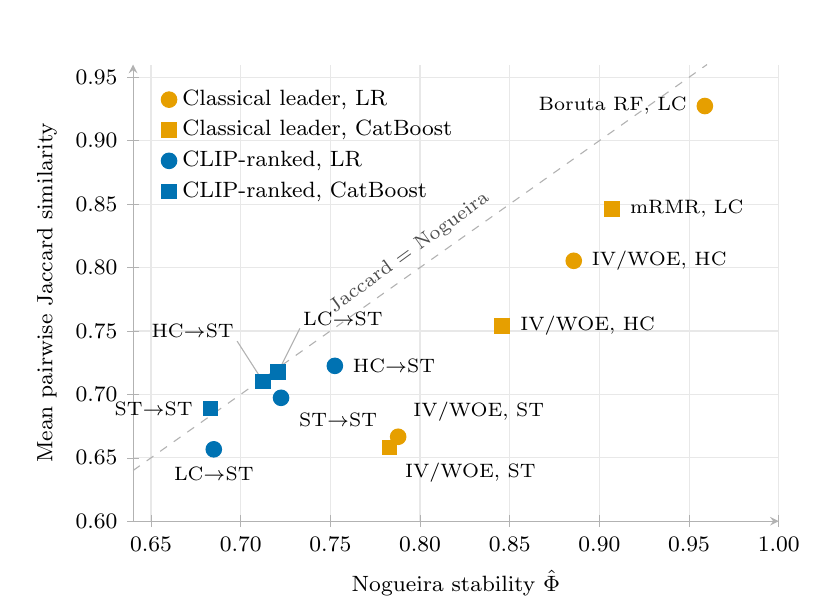
\begin{tikzpicture}
\begin{axis}[
    paper,
    scale only axis, width=8.2cm, height=5.8cm,
    axis lines=left, clip=false,
    xlabel={Nogueira stability $\hat\Phi$}, ylabel={Mean pairwise Jaccard similarity},
    xmin=0.64, xmax=1.00, ymin=0.60, ymax=0.96,
    xtick={0.65,0.70,0.75,0.80,0.85,0.90,0.95,1.00},
    ytick={0.60,0.65,0.70,0.75,0.80,0.85,0.90,0.95},
    xticklabel style={/pgf/number format/fixed, /pgf/number format/precision=2, /pgf/number format/zerofill},
    yticklabel style={/pgf/number format/fixed, /pgf/number format/precision=2, /pgf/number format/zerofill},
    xmajorgrids, ymajorgrids,
    legend pos=north west, legend cell align=left,
]
\addplot[domain=0.64:0.96, samples=2, dashed, gray!60, forget plot] {x};
\node[font=\scriptsize, gray!60!black, rotate=36, anchor=south] at (axis cs:0.80,0.80) {Jaccard $=$ Nogueira};
\addplot[only marks, mark=*, mark size=2.8pt, cOrange]
    coordinates {(0.8857,0.8053) (0.9588,0.9273) (0.7878,0.6666)};
\addlegendentry{Classical leader, LR}
\addplot[only marks, mark=square*, mark size=2.6pt, cOrange]
    coordinates {(0.8458,0.7538) (0.9070,0.8462) (0.7831,0.6582)};
\addlegendentry{Classical leader, CatBoost}
\addplot[only marks, mark=*, mark size=2.8pt, cBlue]
    coordinates {(0.7225,0.6973) (0.7525,0.7225) (0.6850,0.6567)};
\addlegendentry{CLIP-ranked, LR}
\addplot[only marks, mark=square*, mark size=2.6pt, cBlue]
    coordinates {(0.6833,0.6889) (0.7125,0.7101) (0.7208,0.7175)};
\addlegendentry{CLIP-ranked, CatBoost}
\node[font=\scriptsize, anchor=west, xshift=3pt] at (axis cs:0.8857,0.8053) {IV/WOE, HC};
\node[font=\scriptsize, anchor=west, xshift=3pt] at (axis cs:0.8458,0.7538) {IV/WOE, HC};
\node[font=\scriptsize, anchor=east, xshift=-3pt] at (axis cs:0.9588,0.9273) {Boruta RF, LC};
\node[font=\scriptsize, anchor=west, xshift=3pt] at (axis cs:0.9070,0.8462) {mRMR, LC};
\node[font=\scriptsize, anchor=south west, xshift=2pt, yshift=2pt] at (axis cs:0.7878,0.6666) {IV/WOE, ST};
\node[font=\scriptsize, anchor=north west, xshift=2pt, yshift=-2pt] at (axis cs:0.7831,0.6582) {IV/WOE, ST};
\node[font=\scriptsize, anchor=north west, xshift=3pt, yshift=-2pt] at (axis cs:0.7225,0.6973) {ST$\rightarrow$ST};
\node[font=\scriptsize, anchor=east, xshift=-3pt] at (axis cs:0.6833,0.6889) {ST$\rightarrow$ST};
\node[font=\scriptsize, anchor=west, xshift=3pt] at (axis cs:0.7525,0.7225) {HC$\rightarrow$ST};
\draw[gray!60, thin] (axis cs:0.7125,0.7101) -- (axis cs:0.6980,0.7420);
\node[font=\scriptsize, anchor=south east, inner sep=1pt] at (axis cs:0.6980,0.7420) {HC$\rightarrow$ST};
\node[font=\scriptsize, anchor=north, yshift=-3pt] at (axis cs:0.6850,0.6567) {LC$\rightarrow$ST};
\draw[gray!60, thin] (axis cs:0.7208,0.7175) -- (axis cs:0.7330,0.7520);
\node[font=\scriptsize, anchor=south west, inner sep=1pt] at (axis cs:0.7330,0.7520) {LC$\rightarrow$ST};
\end{axis}
\end{tikzpicture}
\caption{Reproducibility landscape of fold-level selections. Orange: most reproducible refitted classical selector in each dataset--backbone case; blue: CLIP-ranked cells on Stability 2024, labelled source$\rightarrow$target. Circles are logistic regression ($\Kfeat=20$), squares CatBoost ($\Kfeat=40$). HC = Home Credit, LC = LendingClub v2, ST = Stability 2024. Higher is more reproducible on both axes; the dashed line marks equality of the two statistics. The Nogueira universe is the eligible universe for the classical leaders and the 60- or 100-feature candidate pool for the CLIP cells, so the two groups are not on a common scale.}
\label{fig:stability}
\end{figure*}

\subsection{CLIP Results}
\label{subsec:clip_results}

Table~\ref{tab:clip_cells} and Figure~\ref{fig:clip}a report the six CLIP-ranked cells on the earlier Stability 2024 OOT cohort (cutoff 2020-02-26; Section~\ref{subsec:dev_oot}), the transfer experiment of RQ3. The native Stability representation with CatBoost is the best cell (0.7729), followed by the Home Credit source (0.7620) and the LendingClub source (0.7503), and CatBoost exceeds logistic regression under every source; for logistic regression the Home Credit source ranking (0.7064) is 0.0287 above the native ranking (0.6777) and the LendingClub source (0.6679) is 0.0099 below it. Across the six cells OOT KS ranges from 0.240 to 0.412, Lift@10 from 2.51 to 3.71 and Capture@10 from 0.251 to 0.371. All six OOT values lie $+0.016$ to $+0.045$ above the pooled DEV out-of-fold AUC. This is an observation about these cells rather than an established mechanism: differences in composition between the fold-validation populations and the OOT cohort, the larger training set of the full-DEV refit compared with the fold models, and other differences between the two evaluations are possible explanations, and the comparison does not by itself rule out optimism in this branch. These values describe the whole pipeline of contrastive ranking, RF/correlation filter and target-trained classifier, and they lie 0.08 to 0.17 below the pure LLM and best classical selectors of Table~\ref{tab:primary_results} (0.8344 and 0.8030 for logistic regression, 0.8784 and 0.8500 for CatBoost), which were scored on the 2020-02-01 cohort, so the comparison crosses cohorts and is descriptive; this gap is why the contrastive branch is evaluated on reproducibility and portability rather than on maximum discrimination. Score PSI is below 0.04 in five of the six cells; the Home Credit source with CatBoost, at 0.1536, is the exception.

\begin{table*}[htbp]
\centering
\footnotesize
\begin{threeparttable}
\caption{CLIP-ranked cells on the earlier Stability 2024 cohort (OOT from 2020-02-26; 304,916 decisions; 8,349 events; see the note to Table~\ref{tab:datasets}), not the headline cohort: development fold AUC (mean and standard deviation over the five folds), pooled DEV out-of-fold AUC and locked-OOT metrics, including score PSI against the DEV reference. $P$ is the pool passed to the RF/correlation filter.}
\label{tab:clip_cells}
\begin{tabular}{@{}llrrlrrrrrr@{}}
\toprule
Source & Model & $P$ & $\Kfeat$ & Fold AUC (SD) & OOF AUC & OOT AUC & KS & Lift@10 & Capture@10 & Score PSI \\
\midrule
Stability & LR & 60 & 20 & 0.6542 (0.0060) & 0.6567 & 0.6777 & 0.269 & 2.67 & 0.267 & 0.0216 \\
Stability & CatBoost & 100 & 40 & 0.7516 (0.0198) & 0.7560 & 0.7729 & 0.412 & 3.71 & 0.371 & 0.0105 \\
Home Credit & LR & 60 & 20 & 0.6728 (0.0093) & 0.6729 & 0.7064 & 0.309 & 2.81 & 0.281 & 0.0335 \\
Home Credit & CatBoost & 100 & 40 & 0.7465 (0.0129) & 0.7459 & 0.7620 & 0.388 & 3.55 & 0.355 & 0.1536 \\
LendingClub & LR & 60 & 20 & 0.6182 (0.0120) & 0.6227 & 0.6679 & 0.240 & 2.51 & 0.251 & 0.0207 \\
LendingClub & CatBoost & 100 & 40 & 0.7222 (0.0128) & 0.7257 & 0.7503 & 0.372 & 3.59 & 0.359 & 0.0075 \\
\bottomrule
\end{tabular}
\end{threeparttable}
\end{table*}

\begin{figure*}[htbp]
\centering
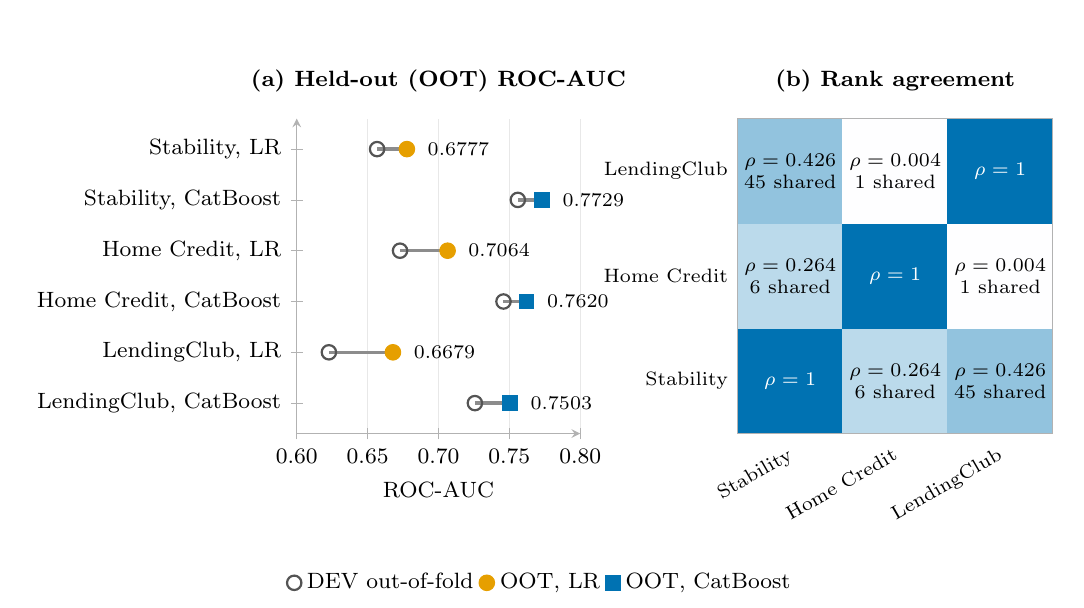
\begin{tikzpicture}
\begin{groupplot}[
    paper,
    group style={group size=2 by 1, horizontal sep=20mm},
    scale only axis, height=4.0cm, clip=false,
]
\nextgroupplot[
    title={(a) Held-out (OOT) ROC-AUC},
    width=3.6cm, axis lines=left, xmajorgrids,
    xlabel={ROC-AUC}, xmin=0.60, xmax=0.80, xtick={0.60,0.65,0.70,0.75,0.80},
    xticklabel style={/pgf/number format/fixed, /pgf/number format/precision=2, /pgf/number format/zerofill},
    ymin=0.4, ymax=6.6, ytick={1,2,3,4,5,6},
    yticklabels={{LendingClub, CatBoost},{LendingClub, LR},{Home Credit, CatBoost},{Home Credit, LR},{Stability, CatBoost},{Stability, LR}},
    legend to name=cliplegend, legend columns=3,
]
\addplot[cGrey, line width=1.2pt, forget plot] coordinates {(0.656681,6) (0.677712,6)};
\addplot[cGrey, line width=1.2pt, forget plot] coordinates {(0.755978,5) (0.772872,5)};
\addplot[cGrey, line width=1.2pt, forget plot] coordinates {(0.672869,4) (0.706434,4)};
\addplot[cGrey, line width=1.2pt, forget plot] coordinates {(0.745859,3) (0.761999,3)};
\addplot[cGrey, line width=1.2pt, forget plot] coordinates {(0.622680,2) (0.667862,2)};
\addplot[cGrey, line width=1.2pt, forget plot] coordinates {(0.725691,1) (0.750327,1)};
\addplot[only marks, mark=o, mark size=2.6pt, thick, cGrey!60!black]
    coordinates {(0.656681,6) (0.755978,5) (0.672869,4) (0.745859,3) (0.622680,2) (0.725691,1)};
\addlegendentry{DEV out-of-fold}
\addplot[only marks, mark=*, mark size=2.8pt, cOrange] coordinates {(0.677712,6) (0.706434,4) (0.667862,2)};
\addlegendentry{OOT, LR}
\addplot[only marks, mark=square*, mark size=2.6pt, cBlue] coordinates {(0.772872,5) (0.761999,3) (0.750327,1)};
\addlegendentry{OOT, CatBoost}
\node[font=\scriptsize, anchor=west, xshift=4pt] at (axis cs:0.6777,6) {0.6777};
\node[font=\scriptsize, anchor=west, xshift=4pt] at (axis cs:0.772872,5) {0.7729};
\node[font=\scriptsize, anchor=west, xshift=4pt] at (axis cs:0.7064,4) {0.7064};
\node[font=\scriptsize, anchor=west, xshift=4pt] at (axis cs:0.761999,3) {0.7620};
\node[font=\scriptsize, anchor=west, xshift=4pt] at (axis cs:0.6679,2) {0.6679};
\node[font=\scriptsize, anchor=west, xshift=4pt] at (axis cs:0.750327,1) {0.7503};
\nextgroupplot[
    title={(b) Rank agreement},
    width=4.0cm,
    xmin=-0.5, xmax=2.5, ymin=-0.5, ymax=2.5,
    xtick={0,1,2}, xticklabels={Stability,Home Credit,LendingClub},
    ytick={0,1,2}, yticklabels={Stability,Home Credit,LendingClub},
    x tick label style={rotate=30, anchor=north east, font=\scriptsize},
    y tick label style={font=\scriptsize},
    tick style={draw=none}, enlargelimits=false, axis on top,
    colormap={paperblue}{color=(white) color=(cBlue)},
    point meta min=0, point meta max=1,
]
\addplot[matrix plot*, mesh/cols=3, point meta=explicit] coordinates {
    (0,0) [1] (1,0) [0.264] (2,0) [0.426]
    (0,1) [0.264] (1,1) [1] (2,1) [0.004]
    (0,2) [0.426] (1,2) [0.004] (2,2) [1]
};
\node[font=\scriptsize, white] at (axis cs:0,0) {$\rho=1$};
\node[font=\scriptsize, white] at (axis cs:1,1) {$\rho=1$};
\node[font=\scriptsize, white] at (axis cs:2,2) {$\rho=1$};
\node[font=\scriptsize, align=center] at (axis cs:1,0) {$\rho=0.264$\\6 shared};
\node[font=\scriptsize, align=center] at (axis cs:0,1) {$\rho=0.264$\\6 shared};
\node[font=\scriptsize, align=center] at (axis cs:2,0) {$\rho=0.426$\\45 shared};
\node[font=\scriptsize, align=center] at (axis cs:0,2) {$\rho=0.426$\\45 shared};
\node[font=\scriptsize, align=center] at (axis cs:2,1) {$\rho=0.004$\\1 shared};
\node[font=\scriptsize, align=center] at (axis cs:1,2) {$\rho=0.004$\\1 shared};
\end{groupplot}
\node[anchor=north, yshift=-2mm] at (current bounding box.south) {\pgfplotslegendfromname{cliplegend}};
\end{tikzpicture}
\caption{CLIP-ranked selection on Stability 2024. (a) Held-out (OOT) ROC-AUC of the six source--backbone cells on the earlier Stability cohort; the hollow marker is the pooled DEV out-of-fold AUC, so the grey bar shows the difference between the OOT value and the development estimate. (b) Spearman correlation over all 1,959 features between the rankings produced by the three source representations, with the number of features shared by the two top-100 lists; the colour scale runs from 0 (white) to 1 (blue), the diagonal shows the self-correlation of 1, and darker cells indicate closer agreement.}
\label{fig:clip}
\end{figure*}

The three source representations do not produce one universal ordering of the Stability predictors (Figure~\ref{fig:clip}b): the native Stability ranking shares only 6 of its top 100 features with the Home Credit ranking (Spearman $\rho=0.264$) and 45 with the LendingClub ranking ($\rho=0.426$), and Home Credit and LendingClub share a single feature ($\rho=0.004$). Transfer is therefore source-dependent. A possible explanation is that each source carries its own descriptor transform, projection geometry and anchor, so the same features are scored through different coordinate systems; the target-aware redundancy stage and classifier then operate on pools that differ substantially between sources. These cells are separate source--target evaluations: the earlier experiments in which the same sources ranked Home Credit features (0.7627 for the Home Credit source with CatBoost; 0.6766 and 0.5732 for the LendingClub source with CatBoost and logistic regression) concern a different target dataset, so the Stability values (0.7620; 0.7503 and 0.6679) show neither that a representation stayed unchanged nor that it improved. The five native seeds are homogeneous (validation mean reciprocal rank 0.2255 to 0.2651 over 395 held-out pairs, Recall@10 0.472 to 0.546, cosine margin 0.528 to 0.568, all collapse checks passed), and score PSI is below 0.10 in five of six cells, with moderate drift for the Home Credit source with CatBoost (0.153625). Finally, the reason for assessing the branch on reproducibility is visible in its earlier Home Credit evaluation (Table~\ref{tab:stages}): inserting the corrected contrastive ranking between LLM screening and mRMR changed OOT AUC by $-0.001102$ (logistic regression) and $+0.000866$ (CatBoost) while raising mean pairwise Jaccard by $+0.324841$ and $+0.498638$ and lowering CatBoost score PSI from 0.008286 to 0.004094; a possible explanation is that the representation imposes a consistent ordering inside a pool that already contains the strong predictors.

\subsection{Voting Results}
\label{subsec:voting_results}

Table~\ref{tab:voting} and Figure~\ref{fig:voting} compare the eight Home Credit voting variants (RQ4) with the sequential pipeline LLM then mRMR that they are designed to improve on, and with full-pool mRMR applied to all 529 features. Voting exceeds the sequential comparator in five of eight point estimates and never exceeds the full-pool reference. Among the pool-based variants AUC rises monotonically with the pool size $P$ for both backbones, from 0.7394 at $P=100$ to 0.7447 at $P=300$ for logistic regression and from 0.7588 to 0.7664 for CatBoost. The logistic-regression gains at $P=200$ and $P=300$ ($+0.0059$ and $+0.0066$) and the CatBoost gain at $P=300$ ($+0.0035$) are Holm-significant within the 24-test voting family, whereas the CatBoost $P=100$ and direct three-voter variants are significantly below the sequential comparator; the direct three-voter selector is weaker than the best pool-based variant under both backbones. Against full-pool mRMR all eight point estimates are negative: for CatBoost, whose reference is the same mutual-information selector as in the headline tables, the deficits at $P=100$, $P=200$ and for the direct variant ($-0.0081$, $-0.0076$ and $-0.0123$) are Holm-significant while the $P=300$ deficit of $0.000391$ is not ($p=0.618$), and for logistic regression the deficits against the final full-pool reference are $0.025$ to $0.030$ and were not tested. Against the third comparator, LLM then CLIP then mRMR, five of eight differences are positive and three of them significant. In terms of AUC, parallel aggregation of the semantic and contrastive rankings therefore exceeds the sequential pipeline by up to $+0.0066$ (logistic regression) and $+0.0035$ (CatBoost) at $P=300$, while remaining $0.025$ to $0.030$ below full-pool mRMR for logistic regression and $0.0004$ to $0.012$ below it for CatBoost; these are AUC differences and do not measure information recovered.

\begin{table*}[htbp]
\centering
\scriptsize
\setlength{\tabcolsep}{3pt}
\begin{threeparttable}
\caption{Home Credit voting experiment. Pool variants average the normalised LLM and contrastive ranks, keep the top $P$ features and apply mutual-information mRMR; the direct variant averages LLM, contrastive and mRMR relevance ranks and selects $\Kfeat$ directly. $\Delta$ is voting minus the sequential comparator (LLM then mRMR); $p$-values are Holm-adjusted within the family of 24 voting tests. AUC is shown to four decimals and $\Delta$ at full precision.}
\label{tab:voting}
\begin{tabular}{@{}lrrlrrl@{}}
\toprule
 & \multicolumn{3}{c}{Logistic regression, $\Kfeat=20$} & \multicolumn{3}{c}{CatBoost, $\Kfeat=40$} \\
\cmidrule(lr){2-4}\cmidrule(l){5-7}
Variant & AUC & $\Delta$ & Holm $p$ & AUC & $\Delta$ & Holm $p$ \\
\midrule
Pool $P=100$, then mRMR & 0.7394 & $+0.001334$ & 0.386 & 0.7588 & $-0.004197$ & 0.041 \\
Pool $P=200$, then mRMR & 0.7440 & $+0.005921$ & $3.7\times10^{-8}$ & 0.7593 & $-0.003691$ & 0.064 \\
Pool $P=300$, then mRMR & 0.7447 & $+0.006554$ & $1.7\times10^{-10}$ & 0.7664 & $+0.003495$ & 0.042 \\
Direct three-voter & 0.7406 & $+0.002474$ & 0.122 & 0.7545 & $-0.008433$ & $5.7\times10^{-7}$ \\
\midrule
Sequential LLM then mRMR & 0.7381 & & & 0.7630 & & \\
Full-pool mRMR (529 features) & 0.7699 & & & 0.7668 & & \\
\bottomrule
\end{tabular}
\end{threeparttable}
\end{table*}

\begin{figure*}[htbp]
\centering
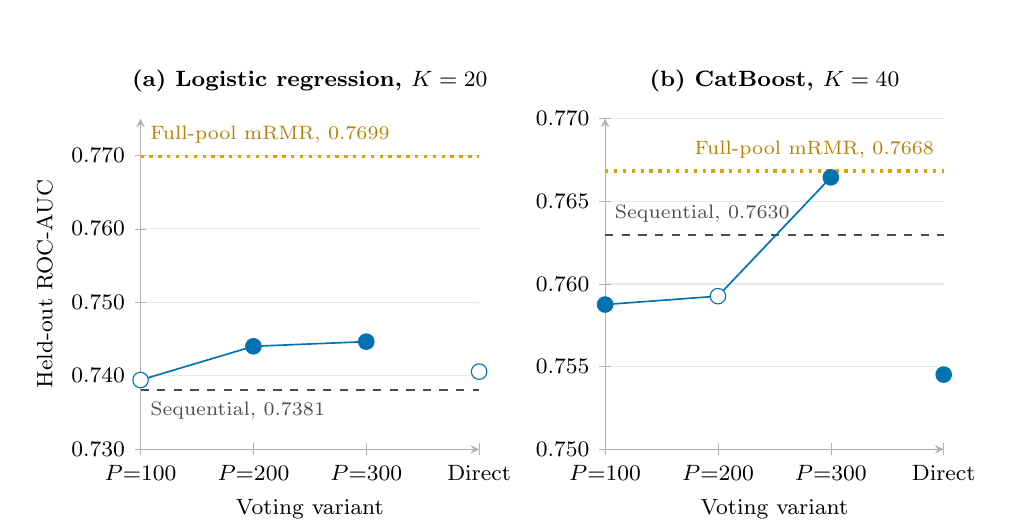
\begin{tikzpicture}
\begin{groupplot}[
    paper,
    group style={group size=2 by 1, horizontal sep=16mm},
    scale only axis, width=4.3cm, height=4.2cm, clip=false,
    symbolic x coords={100,200,300,Direct},
    xtick={100,200,300,Direct}, xticklabels={$P{=}100$,$P{=}200$,$P{=}300$,Direct},
    enlarge x limits=0.22, ymajorgrids, axis lines=left,
    yticklabel style={/pgf/number format/fixed, /pgf/number format/precision=3, /pgf/number format/zerofill},
    xlabel={Voting variant},
]
\nextgroupplot[title={(a) Logistic regression, $\Kfeat=20$}, ylabel={Held-out ROC-AUC}, ymin=0.730, ymax=0.775, ytick distance=0.010]
\addplot[dashed, thick, gray!60!black] coordinates {(100,0.738098) (Direct,0.738098)};
\addplot[dotted, very thick, cOrange] coordinates {(100,0.769890) (Direct,0.769890)};
\addplot[cBlue, semithick, mark=none] coordinates {(100,0.739432) (200,0.744020) (300,0.744653)};
\addplot[only marks, mark=*, mark size=2.8pt, cBlue] coordinates {(200,0.744020) (300,0.744653)};
\addplot[only marks, mark=*, mark size=2.8pt, cBlue, fill=white] coordinates {(100,0.739432) (Direct,0.740573)};
\node[font=\scriptsize, anchor=north west, gray!60!black] at (axis cs:100,0.738098) [yshift=-1pt] {Sequential, 0.7381};
\node[font=\scriptsize, anchor=south west, cOrange!80!black] at (axis cs:100,0.769890) [yshift=1pt] {Full-pool mRMR, 0.7699};
\nextgroupplot[title={(b) CatBoost, $\Kfeat=40$}, ymin=0.750, ymax=0.770, ytick distance=0.005]
\addplot[dashed, thick, gray!60!black] coordinates {(100,0.762954) (Direct,0.762954)};
\addplot[dotted, very thick, cOrange] coordinates {(100,0.766839) (Direct,0.766839)};
\addplot[cBlue, semithick, mark=none] coordinates {(100,0.758757) (200,0.759263) (300,0.766448)};
\addplot[only marks, mark=*, mark size=2.8pt, cBlue] coordinates {(100,0.758757) (300,0.766448) (Direct,0.754521)};
\addplot[only marks, mark=*, mark size=2.8pt, cBlue, fill=white] coordinates {(200,0.759263)};
\node[font=\scriptsize, anchor=south west, gray!60!black] at (axis cs:100,0.762954) [yshift=1pt] {Sequential, 0.7630};
\node[font=\scriptsize, anchor=south east, cOrange!80!black] at (axis cs:Direct,0.766839) [yshift=1pt] {Full-pool mRMR, 0.7668};
\end{groupplot}
\end{tikzpicture}
\caption{Home Credit voting AUC by candidate-pool size for (a) logistic regression and (b) CatBoost. Filled markers are Holm-significant differences from the sequential comparator (dashed line) within the 24-test voting family; hollow markers are not significant. The dotted line is full-pool mRMR on all 529 features. The vertical scales differ between panels.}
\label{fig:voting}
\end{figure*}

\paragraph{Scalability and cost of the pre-screening stage}
The largest dataset has 1,157,512 development decisions and 1,959 engineered features held as a sparse matrix, and the pre-screening stage scales with the number of features rather than the number of rows: one cached ranking per dataset serves every fold and both backbones, whereas mutual-information mRMR must estimate relevance for every candidate and redundancy for every candidate pair on every fold. In the development experiments on Home Credit and LendingClub, 72 logical screening requests were served by 24 provider ranking calls and 48 cache hits, with 6 further calls generating source descriptions; the 30 physical calls consumed 806,757 input and 56,495 output tokens, for a direct API cost bounded between USD~0.171 and USD~0.413 at the rates in force (USD~0.625 to 1.396 without caching). Total pipeline time on Home Credit logistic regression was 0.8 minutes for pure LLM against 12.1 minutes for full-pool mRMR and 24.6 minutes for stable core plus LLM fill; on LendingClub CatBoost, model fitting dominated and every pipeline took 65 to 74 minutes except stable core plus LLM fill (256 minutes). Runtimes were measured under unequal caching and execution conditions and are descriptive only; the final three-dataset run was not separately metered.

% ============================================================
% 7. DISCUSSION
% ============================================================

\section{Discussion}
\label{sec:discussion}

\subsection{Main Findings}
\label{subsec:main_findings}

RQ1 asked whether an LLM pre-screened subset can match or exceed classically selected subsets on held-out data under a fixed budget. The answer is conditional: in five of six dataset--backbone cases the best LLM-assisted selector attains a significantly higher held-out ROC-AUC than the best classical selector, and in every same-cohort comparison but one the best compact subset also has a higher point estimate than the full-feature model, whereas on Home Credit logistic regression mutual-information mRMR exceeds the best LLM-assisted pipeline by 0.021. The leading LLM-assisted method is pure LLM in four cases, LLM then mRMR in one (LendingClub v2 CatBoost) and stable core plus LLM fill in the Home Credit logistic-regression case that the classical selector wins. Within these comparisons the semantic ranking was therefore most often effective when used directly; statistical refinement of the semantic pool led in one case, and on Home Credit CatBoost it reduced held-out AUC from 0.7935 (pure LLM) to 0.7630 (LLM then mRMR, Table~\ref{tab:voting}). Direct use of the semantic ranking and statistical refinement are alternatives whose value depends on the dataset and backbone; the results do not establish either arrangement as generally preferable, nor LLM pre-screening as a replacement for statistical selection. On reproducibility (RQ2), refitted classical selectors reach Nogueira stability between 0.78 and 0.96, with information value and Boruta the most reproducible, and the contrastive ranking followed by the RF/correlation filter reaches 0.68 to 0.75 when computed over its candidate pools of 60 or 100 features, a universe not comparable with the classical one; in the earlier Home Credit experiments, inserting the representation into an LLM-screened pipeline raised fold-to-fold Jaccard similarity by 0.32 to 0.50 while OOT AUC changed by less than 0.002, an observation consistent with reproducibility and discrimination being separable outcomes. On portability (RQ3), representations trained on three portfolios rank the same Stability predictors very differently, and every transferred ranking supports a model whose OOT AUC exceeds its development estimate, an observation discussed in Section~\ref{subsec:clip_results}; each source--target cell is a separate evaluation and is not compared with the earlier Home Credit target. On the order of combination (RQ4), parallel rank voting exceeds sequential screening in five of eight point estimates, three of them significantly, but never exceeds mRMR on the full universe. On Home Credit, the only dataset in the voting experiment, the size of the pool given to the statistical stage therefore mattered more than the order of the semantic and statistical stages; the manuscript does not establish this as a general rule.

\subsection{Predictive Performance vs Stability}
\label{subsec:performance_vs_stability}

Three trade-offs emerge. The LLM-assisted pipelines that lead discrimination on LendingClub and Stability rest on a fixed cached ranking whose fold agreement is perfect by construction; their reproducibility as deployed selectors depends on the language model under a fixed snapshot and prompt, which the study controls by caching rather than by repeated calls. The classical selectors that lead reproducibility (IV/WOE, Boruta RF) are not those that lead discrimination (RFE CatBoost, IV then Boruta, mRMR), which are wrappers or greedy procedures; greater sensitivity to the training sample is a possible explanation. The contrastive representation, in the earlier Home Credit experiments, and the stable-core construction are the two devices intended to raise the reproducibility of a semantically screened subset; the stable-core hybrid is the best LLM-assisted pipeline on Home Credit logistic regression, although it remains below mRMR there, and its own fold stability is not reported. CatBoost exceeds logistic regression in every headline case, but the two backbones differ in both model class and feature budget (40 against 20), so the difference cannot be attributed to either factor alone; the development observation that the boosted model was less sensitive to redundant predictors (Section~\ref{subsec:feature_budgets}) is consistent with, but does not establish, a general budget effect. Held-out drift is low for the leading pipelines, with the lowest score PSI per dataset below 0.001 and zero median feature PSI for the pure LLM subsets on Home Credit, although these are minima, one CLIP-ranked cell reaches a score PSI of 0.153625, and lower feature drift does not translate mechanically into lower score drift or better discrimination.

\subsection{Cross-Dataset Behavior}
\label{subsec:cross_dataset}

Several findings reproduce across datasets and backbones: the best compact subset exceeds the full-feature model in every same-cohort case except Home Credit logistic regression (the two Stability 2024 references belong to the earlier cohort, Section~\ref{subsec:dev_oot}); CatBoost at its budget of 40 features exceeds logistic regression at 20 in every headline case, for every full-feature reference and in every CLIP-ranked cell, a difference that combines model class and budget; an LLM-assisted CatBoost pipeline attains the highest KS and the lowest Brier score among the evaluated selectors in all three datasets, and a classical wrapper the best top-decile concentration; and the lowest score PSI in each dataset is below 0.001. Other findings are dataset- or model-specific: the direction of the headline comparison reverses on Home Credit logistic regression; the best classical comparator changes identity across cases; the LLM-assisted gain is largest on LendingClub, where eligibility screening removes most of the universe and the resolved-outcome population has the highest event rate, and smallest on Home Credit CatBoost; and contrastive transfer depends on the source--target pair rather than on the source alone; the shared institutional lineage of Home Credit and Stability 2024 is a possible, not a demonstrated, explanation for the Home Credit source's performance there. The Stability 2024 OOT window, February to October 2020, overlaps the onset of the COVID-19 pandemic; the study does not establish what that period did to the portfolio, and portfolio-specific interventions in it are a possible influence on the reported magnitudes, so the Stability results should not be read as demonstrated robustness to a regime shift. Generalisation from these three public portfolios to other lenders is therefore plausible for the qualitative conclusions and uncertain for the magnitudes.

\subsection{Limitations}
\label{subsec:limitations}

The datasets are public releases with provider-defined targets whose horizons are not fully specified; Home Credit is ordered by the recency of the applicant's most recent previous application rather than by calendar time, so its held-out population is a recency-based covariate-shift holdout of applicants with a qualifying previous application and its results do not extend to applicants without one; LendingClub time is the issue month, and its population contains resolved loans only, with the selection effects described in Section~\ref{subsec:dev_oot}; and Home Credit and Stability 2024 share institutional lineage, so the study does not contain three independent lenders. The Stability 2024 OOT cutoff was moved once during the study, from 2020-02-26 to 2020-02-01, with knowledge of the event rates of the two populations (Section~\ref{subsec:dev_oot}), and the contrastive extension and the Stability full-feature references were not re-run on the final cohort. The language model's training data very likely include the public data dictionaries, forum discussions and winning-solution write-ups of the Home Credit and LendingClub competitions, so part of its ranking may reflect memorised public knowledge of which variables predict default rather than reasoning from feature meaning; the definition-only contract on Stability 2024, whose engineered features and approved definitions are specific to this study, reduces but does not remove that exposure, and results on proprietary variable books may differ. Two backbones with one fixed configuration each are used, not tuned per selector, with balanced class weights and no recalibration, so probability metrics compare selectors within a dataset only. The two prompt contracts differ by dataset, which prevents attribution to a single semantic algorithm; the LLM ranking is a cached artefact of one model snapshot whose run-to-run variability was not measured; and stability comparisons are confined to refitted selectors. The contrastive representation is built from frozen full-DEV statistics and not recomputed inside each row fold, so its development scores are diagnostic and the locked OOT evaluation is decisive for that branch; the contrastive branch is compared with the headline selectors descriptively only; and the voting experiment covers Home Credit only. With OOT populations of 120,000 to 369,000 observations small AUC differences are statistically detectable, so effect sizes matter more than $p$-values, and inference is confined to the prespecified selector comparisons and the voting family. The study does not evaluate profit, fairness, explanation stability or production deployment, and its cost figures are development-stage measurements at historical prices.

% ============================================================
% 8. CONCLUSION
% ============================================================

\section{Conclusion}
\label{sec:conclusion}

This paper asked whether semantic pre-screening, by a large language model or a contrastive feature representation that reads the variable book but no outcome, can select compact, competitive and governable feature subsets for big-data credit scoring, and how such subsets compare with classical selection under temporal and covariate-shift validation. Across three credit portfolios and two backbones, with fixed budgets of 20 and 40 original features and every development decision frozen before the held-out population was scored, LLM-assisted selection achieved significantly higher held-out ROC-AUC than the best classical selector in five of six cases, with paired gains between $+0.012$ and $+0.051$, and the best compact subset had a higher point estimate than the full-feature model in every same-cohort comparison except one; Home Credit logistic regression was the exception in both respects, with mutual-information mRMR the strongest selector there. Pure LLM was the leading LLM-assisted method in four of the six cases, LLM then mRMR in one and stable core plus LLM fill in the case the classical selector won. Reproducibility, drift and portability were reported as separate outcomes: refitted classical selectors were the most reproducible; in the earlier Home Credit experiments a CLIP-style contrastive representation raised the fold-to-fold Jaccard similarity of semantically screened subsets while OOT AUC changed by less than 0.002, and its rankings transferred across portfolios in a source-dependent way; and parallel rank voting exceeded sequential screening in five of eight point estimates without surpassing statistical selection from the complete universe.

For practice, the results support treating a language model's ranking as a pre-screener for a large engineered variable book, whose cost is set by the number of features rather than the number of decisions, used either directly or as a pool for statistical refinement, with the choice validated per dataset and backbone on held-out data, and with the semantic stage governed by an explicit information contract, a cached ranking and the same freeze, drift and stability monitoring applied to any other selector. For research, they argue for reporting discrimination, subset reproducibility, drift and transfer separately and for locked held-out evaluation, temporal where the data allow it, whenever feature selection is compared. Extending the evaluation to additional lenders, to repeated LLM runs and to profit- and fairness-aware objectives are natural next steps.

% ============================================================
% END MATTER
% ============================================================

\section*{CRediT authorship contribution statement}
\textbf{Dilshod A'zamjonov:} Methodology, Software, Validation, Formal analysis, Investigation, Data curation, Visualization, Writing -- original draft. \textbf{Sejuti Rahman:} Conceptualization, Resources, Supervision, Project administration, Writing -- review \& editing.

\section*{Funding}
This research did not receive any specific grant from funding agencies in the public, commercial, or not-for-profit sectors.

\section*{Disclaimer}
The views expressed in this paper are those of the authors and do not necessarily reflect those of the Central Bank of the Republic of Uzbekistan. The study uses public datasets only; no data of the Central Bank or of any supervised institution were used.

\section*{Declaration of competing interest}
The authors declare that they have no known competing financial interests or personal relationships that could have appeared to influence the work reported in this paper.

\section*{Data availability}
The three datasets are publicly available on Kaggle, and their redistribution is governed by the terms of the respective competitions and dataset licences:
\begin{itemize}
    \item Home Credit Default Risk: \url{https://www.kaggle.com/competitions/home-credit-default-risk/data}
    \item All Lending Club loan data: \url{https://www.kaggle.com/datasets/wordsforthewise/lending-club}
    \item Home Credit -- Credit Risk Model Stability: \url{https://www.kaggle.com/competitions/home-credit-credit-risk-model-stability/data}
    \item Code, configuration files, cached rankings and experiment artefacts: \url{https://github.com/dilshodazamjonov/Feature-Selection-Research}
\end{itemize}

\section*{Declaration of generative AI and AI-assisted technologies in the writing process}
During the preparation of this work the authors used Claude (Anthropic) to draft and edit the manuscript text, to typeset tables and figures from the study's result files, and to check reference metadata. After using this tool, the authors reviewed and edited the content as needed and take full responsibility for the content of the published article. The GPT-4.1 mini model described in Section~\ref{subsec:llm_fs} is a component of the feature-selection methods under study and is not part of the writing process.

\appendix
\section{LLM prompt templates}
\label{app:prompts}

Section~\ref{subsec:llm_fs} describes two prompt templates, which are reproduced verbatim below: \ref{app:prompt_v3} gives \texttt{stability\_\allowbreak expert\_\allowbreak v3}, used for Home Credit and LendingClub, and \ref{app:prompt_v5} gives \texttt{stability\_\allowbreak expert\_\allowbreak v5}, used for Stability 2024. The braced fields are rendered at run time with the ranking budget and one line per candidate feature. Under \texttt{stability\_\allowbreak expert\_\allowbreak v3} each feature line carries the name, semantic group, source table, data type, missingness, non-null count, description and, where applicable, numeric summaries or categorical cardinality; under \texttt{stability\_\allowbreak expert\_\allowbreak v5} it carries the approved definition and adapter lineage only.

\subsection{Home Credit and LendingClub prompt}
\label{app:prompt_v3}
\begin{lstlisting}
You are a senior retail credit-risk feature-screening expert.

Context:
- You are reviewing metadata only, the way a strong credit-risk expert would review a variable pack before modeling.
- Your job is to create a broad, stability-aware candidate ranking for downstream model development.
- A downstream statistical selector will make the final redundancy pruning and final budget decision.

Task:
Produce a broad, stability-aware candidate ranking of up to {ranking_budget} features for a binary loan-default model.
Do not try to make the final statistical selection yourself. The downstream selector will refine this list for redundancy and final budget.

Priority criteria:
1. Stable out-of-time generalization.
2. Low missingness and broad coverage.
3. Interpretable credit-risk meaning.
4. Durable repayment behavior, indebtedness, leverage, exposure, utilization, capacity, delinquency, and customer history signals.
5. Avoid leakage-like artifacts, policy/process contamination, brittle operational proxies, and unstable sparse tail-dominated variables.
6. Control redundancy among near-duplicate aggregates, especially within the same semantic group, unless variants clearly add distinct information.
7. Prefer representatives that a credit-risk expert could defend in a stable scorecard review.

Rules:
1. Use only the feature names provided below.
2. You are seeing training-slice metadata only, not validation or OOT data.
3. Prefer broad semantic coverage rather than over-concentrating on one narrow family.
4. When two features look similar, prefer the less-missing, more interpretable, more operationally durable one.
5. Avoid selecting many duplicate aggregates from one business concept unless their summaries suggest meaningfully different information.
6. Return features in priority order, best first.
7. Do not invent new feature names.

Features:
{features_text}

Return ONLY valid JSON:
{
  "selected_features": ["feature_1", "feature_2"],
  "reasoning_summary": "One concise high-level reason.",
  "selection_principles": ["stability", "coverage", "redundancy control"],
  "feature_reasons": {}
}

Keep the response compact. Do not include per-feature explanations unless absolutely necessary.
\end{lstlisting}

\subsection{Stability 2024 prompt}
\label{app:prompt_v5}
\begin{lstlisting}
You are a senior retail credit-risk feature-screening expert.

Context:
- You are reviewing outcome-independent feature definitions and adapter lineage only, the way a strong credit-risk expert would review a variable pack before modeling.
- Your job is to create a broad, stability-aware candidate ranking for downstream model development.
- A downstream statistical selector may perform fold-local supervised stability fitting and final redundancy pruning.

Task:
Produce a broad, stability-aware candidate ranking of exactly {ranking_budget} features for a binary loan-default model.
Do not try to make the final statistical selection yourself. Downstream consumers will apply the frozen model-specific budgets.

Priority criteria:
1. Stable out-of-time generalization.
2. Interpretable credit-risk meaning grounded only in the supplied definitions and lineage.
3. Durable repayment behavior, indebtedness, leverage, exposure, utilization, capacity, delinquency, and customer-history signals.
4. Avoid leakage-like artifacts, policy/process contamination, and brittle operational proxies identifiable from definitions alone.
5. Control redundancy among near-duplicate aggregates, especially within the same source family, unless variants clearly add distinct information.
6. Prefer representatives that a credit-risk expert could defend in a stable scorecard review.

Rules:
1. Use only the feature names provided below and copy every selected name verbatim.
2. You are seeing no rows, targets, split statistics, validation information, OOT information, performance, drift, missingness rates, IV, correlation, mutual information, SHAP, or model importance.
3. Prefer broad semantic coverage rather than over-concentrating on one narrow family.
4. Return exactly {ranking_budget} distinct features in priority order, best first.
5. Every candidate not placed in the {ranking_budget}-item selected_features array is intentionally not selected.
6. Do not return more or fewer than {ranking_budget} names. Do not invent, normalize, replace, or duplicate a selected name.

Features:
{features_text}

Return ONLY valid JSON:
{
  "selected_features": ["feature_1", "feature_2"],
  "reasoning_summary": "One concise high-level reason.",
  "selection_principles": ["stability", "coverage", "redundancy control"],
  "feature_reasons": {}
}

Keep the response compact. Do not include per-feature explanations unless absolutely necessary.
\end{lstlisting}

% ============================================================
% REFERENCES
% ============================================================

% Bibliography generated with BibTeX (elsarticle-num style) from refs.bib
% and embedded here so that pdflatex alone suffices. Set in \footnotesize.
\begingroup\footnotesize
% 8pt entries with unbreakable DOI strings cannot always be justified within badness 1000;
% allow looser lines and report only severe cases
\sloppy\hbadness=10000
\begin{thebibliography}{10}
\expandafter\ifx\csname url\endcsname\relax
  \def\url#1{\texttt{#1}}\fi
\expandafter\ifx\csname urlprefix\endcsname\relax\def\urlprefix{URL }\fi
\expandafter\ifx\csname href\endcsname\relax
  \def\href#1#2{#2} \def\path#1{#1}\fi

\bibitem{thomas2002}
L.~C. Thomas, D.~B. Edelman, J.~N. Crook, Credit Scoring and Its Applications,
  SIAM, Philadelphia, 2002.

\bibitem{siddiqi2006}
N.~Siddiqi, Credit Risk Scorecards: Developing and Implementing Intelligent
  Credit Scoring, John Wiley \& Sons, Hoboken, NJ, 2006.

\bibitem{lessmann2015}
S.~Lessmann, B.~Baesens, H.-V. Seow, L.~C. Thomas, Benchmarking
  state-of-the-art classification algorithms for credit scoring: An update of
  research, European Journal of Operational Research 247~(1) (2015) 124--136.
\newblock \href {https://doi.org/10.1016/j.ejor.2015.05.030}
  {\path{doi:10.1016/j.ejor.2015.05.030}}.

\bibitem{gunnarsson2021}
B.~R. Gunnarsson, S.~vanden Broucke, B.~Baesens, M.~{\'O}skarsd{\'o}ttir,
  W.~Lemahieu, Deep learning for credit scoring: Do or don't?, European Journal
  of Operational Research 295~(1) (2021) 292--305.
\newblock \href {https://doi.org/10.1016/j.ejor.2021.03.006}
  {\path{doi:10.1016/j.ejor.2021.03.006}}.

\bibitem{ballegeer2025}
M.~Ballegeer, M.~Bogaert, D.~F. Benoit, Evaluating the stability of model
  explanations in instance-dependent cost-sensitive credit scoring, European
  Journal of Operational Research 326~(3) (2025) 630--640.
\newblock \href {https://doi.org/10.1016/j.ejor.2025.05.041}
  {\path{doi:10.1016/j.ejor.2025.05.041}}.

\bibitem{guyon2003}
I.~Guyon, A.~Elisseeff, An introduction to variable and feature selection,
  Journal of Machine Learning Research 3 (2003) 1157--1182.

\bibitem{peng2005}
H.~Peng, F.~Long, C.~Ding, Feature selection based on mutual information:
  Criteria of max-dependency, max-relevance, and min-redundancy, IEEE
  Transactions on Pattern Analysis and Machine Intelligence 27~(8) (2005)
  1226--1238.
\newblock \href {https://doi.org/10.1109/TPAMI.2005.159}
  {\path{doi:10.1109/TPAMI.2005.159}}.

\bibitem{kohavi1997}
R.~Kohavi, G.~H. John, Wrappers for feature subset selection, Artificial
  Intelligence 97~(1--2) (1997) 273--324.
\newblock \href {https://doi.org/10.1016/S0004-3702(97)00043-X}
  {\path{doi:10.1016/S0004-3702(97)00043-X}}.

\bibitem{guyon2002}
I.~Guyon, J.~Weston, S.~Barnhill, V.~Vapnik, Gene selection for cancer
  classification using support vector machines, Machine Learning 46~(1--3)
  (2002) 389--422.
\newblock \href {https://doi.org/10.1023/A:1012487302797}
  {\path{doi:10.1023/A:1012487302797}}.

\bibitem{kursa2010}
M.~B. Kursa, W.~R. Rudnicki, Feature selection with the {B}oruta package,
  Journal of Statistical Software 36~(11) (2010) 1--13.
\newblock \href {https://doi.org/10.18637/jss.v036.i11}
  {\path{doi:10.18637/jss.v036.i11}}.

\bibitem{tibshirani1996}
R.~Tibshirani, Regression shrinkage and selection via the lasso, Journal of the
  Royal Statistical Society: Series B (Methodological) 58~(1) (1996) 267--288.
\newblock \href {https://doi.org/10.1111/j.2517-6161.1996.tb02080.x}
  {\path{doi:10.1111/j.2517-6161.1996.tb02080.x}}.

\bibitem{lundberg2017}
S.~M. Lundberg, S.-I. Lee, A unified approach to interpreting model
  predictions, in: Advances in Neural Information Processing Systems 30, 2017,
  pp. 4765--4774.

\bibitem{choi2022}
K.~Choi, C.~Cundy, S.~Srivastava, S.~Ermon, {LMPriors}: Pre-trained language
  models as task-specific priors, arXiv preprint arXiv:2210.12530 (2022).
\newblock \href {https://doi.org/10.48550/arXiv.2210.12530}
  {\path{doi:10.48550/arXiv.2210.12530}}.

\bibitem{jeong2025}
D.~P. Jeong, Z.~C. Lipton, P.~Ravikumar, {LLM-Select}: Feature selection with
  large language models, Transactions on Machine Learning Research (2025),
  arXiv:2407.02694.

\bibitem{li2025sigkdd}
D.~Li, Z.~Tan, H.~Liu, Exploring large language models for feature selection: A
  data-centric perspective, ACM SIGKDD Explorations Newsletter 26~(2) (2025)
  44--53.
\newblock \href {https://doi.org/10.1145/3715073.3715077}
  {\path{doi:10.1145/3715073.3715077}}.

\bibitem{zhang2025llmlasso}
E.~Zhang, R.~Goto, N.~Sagan, J.~Mutter, N.~Phillips, A.~Alizadeh, K.~Lee,
  J.~Blanchet, M.~Pilanci, R.~Tibshirani, {LLM-Lasso}: A robust framework for
  domain-informed feature selection and regularization, arXiv preprint
  arXiv:2502.10648 (2025).
\newblock \href {https://doi.org/10.48550/arXiv.2502.10648}
  {\path{doi:10.48550/arXiv.2502.10648}}.

\bibitem{radford2021}
A.~Radford, J.~W. Kim, C.~Hallacy, A.~Ramesh, G.~Goh, S.~Agarwal, G.~Sastry,
  A.~Askell, P.~Mishkin, J.~Clark, G.~Krueger, I.~Sutskever, Learning
  transferable visual models from natural language supervision, in: Proceedings
  of the 38th International Conference on Machine Learning, PMLR 139, 2021, pp.
  8748--8763.

\bibitem{oord2018}
A.~van~den Oord, Y.~Li, O.~Vinyals, Representation learning with contrastive
  predictive coding, arXiv preprint arXiv:1807.03748 (2018).
\newblock \href {https://doi.org/10.48550/arXiv.1807.03748}
  {\path{doi:10.48550/arXiv.1807.03748}}.

\bibitem{kalousis2007}
A.~Kalousis, J.~Prados, M.~Hilario, Stability of feature selection algorithms:
  a study on high-dimensional spaces, Knowledge and Information Systems 12~(1)
  (2007) 95--116.
\newblock \href {https://doi.org/10.1007/s10115-006-0040-8}
  {\path{doi:10.1007/s10115-006-0040-8}}.

\bibitem{nogueira2018}
S.~Nogueira, K.~Sechidis, G.~Brown, On the stability of feature selection
  algorithms, Journal of Machine Learning Research 18~(174) (2018) 1--54.

\bibitem{homecredit2018}
{Home Credit Group},
  \href{https://www.kaggle.com/competitions/home-credit-default-risk}{Home
  {C}redit {D}efault {R}isk}, Kaggle competition dataset (2018).
\newline\urlprefix\url{https://www.kaggle.com/competitions/home-credit-default-risk}

\bibitem{lendingclub_kaggle}
N.~George,
  \href{https://www.kaggle.com/datasets/wordsforthewise/lending-club}{All
  {L}ending {C}lub loan data}, Kaggle dataset, version 3 (loans issued
  2007--2018 Q4) (2019).
\newline\urlprefix\url{https://www.kaggle.com/datasets/wordsforthewise/lending-club}

\bibitem{homecredit2024}
{Home Credit Group},
  \href{https://www.kaggle.com/competitions/home-credit-credit-risk-model-stability}{Home
  {C}redit -- {C}redit {R}isk {M}odel {S}tability}, Kaggle competition dataset
  (2024).
\newline\urlprefix\url{https://www.kaggle.com/competitions/home-credit-credit-risk-model-stability}

\bibitem{prokhorenkova2018}
L.~Prokhorenkova, G.~Gusev, A.~Vorobev, A.~V. Dorogush, A.~Gulin, {CatBoost}:
  unbiased boosting with categorical features, in: Advances in Neural
  Information Processing Systems 31, 2018, pp. 6638--6648.

\bibitem{openai2025gpt41}
{OpenAI}, \href{https://openai.com/index/gpt-4-1/}{Introducing {GPT-4.1} in the
  {API}}, OpenAI product announcement, 14 April 2025 (2025).
\newline\urlprefix\url{https://openai.com/index/gpt-4-1/}

\bibitem{wang2020minilm}
W.~Wang, F.~Wei, L.~Dong, H.~Bao, N.~Yang, M.~Zhou, {MiniLM}: Deep
  self-attention distillation for task-agnostic compression of pre-trained
  transformers, in: Advances in Neural Information Processing Systems 33, 2020,
  pp. 5776--5788.

\bibitem{reimers2019}
N.~Reimers, I.~Gurevych, Sentence-{BERT}: Sentence embeddings using {S}iamese
  {BERT}-networks, in: Proceedings of the 2019 Conference on Empirical Methods
  in Natural Language Processing and the 9th International Joint Conference on
  Natural Language Processing (EMNLP-IJCNLP), 2019, pp. 3982--3992.
\newblock \href {https://doi.org/10.18653/v1/D19-1410}
  {\path{doi:10.18653/v1/D19-1410}}.

\bibitem{baesens2003}
B.~Baesens, T.~Van~Gestel, S.~Viaene, M.~Stepanova, J.~Suykens, J.~Vanthienen,
  Benchmarking state-of-the-art classification algorithms for credit scoring,
  Journal of the Operational Research Society 54~(6) (2003) 627--635.
\newblock \href {https://doi.org/10.1057/palgrave.jors.2601545}
  {\path{doi:10.1057/palgrave.jors.2601545}}.

\bibitem{maldonado2017}
S.~Maldonado, C.~Bravo, J.~L{\'o}pez, J.~P{\'e}rez, Integrated framework for
  profit-based feature selection and {SVM} classification in credit scoring,
  Decision Support Systems 104 (2017) 113--121.
\newblock \href {https://doi.org/10.1016/j.dss.2017.10.007}
  {\path{doi:10.1016/j.dss.2017.10.007}}.

\bibitem{breiman2001}
L.~Breiman, Random forests, Machine Learning 45~(1) (2001) 5--32.
\newblock \href {https://doi.org/10.1023/A:1010933404324}
  {\path{doi:10.1023/A:1010933404324}}.

\bibitem{boloncanedo2015}
V.~Bol{\'o}n-Canedo, N.~S{\'a}nchez-Maro{\~n}o, A.~Alonso-Betanzos, Recent
  advances and emerging challenges of feature selection in the context of big
  data, Knowledge-Based Systems 86 (2015) 33--45.
\newblock \href {https://doi.org/10.1016/j.knosys.2015.05.014}
  {\path{doi:10.1016/j.knosys.2015.05.014}}.

\bibitem{kuncheva2007}
L.~I. Kuncheva, A stability index for feature selection, in: Proceedings of the
  25th IASTED International Multi-Conference: Artificial Intelligence and
  Applications, Innsbruck, Austria, 2007, pp. 390--395.

\bibitem{saeys2008}
Y.~Saeys, T.~Abeel, Y.~Van~de Peer, Robust feature selection using ensemble
  feature selection techniques, in: Machine Learning and Knowledge Discovery in
  Databases (ECML PKDD 2008), Lecture Notes in Computer Science 5212, 2008, pp.
  313--325.
\newblock \href {https://doi.org/10.1007/978-3-540-87481-2_21}
  {\path{doi:10.1007/978-3-540-87481-2_21}}.

\bibitem{dwork2001}
C.~Dwork, R.~Kumar, M.~Naor, D.~Sivakumar, Rank aggregation methods for the
  {W}eb, in: Proceedings of the 10th International Conference on World Wide Web
  (WWW 2001), 2001, pp. 613--622.
\newblock \href {https://doi.org/10.1145/371920.372165}
  {\path{doi:10.1145/371920.372165}}.

\bibitem{sanzguerrero2025}
M.~Sanz-Guerrero, J.~Arroyo, Credit risk meets large language models: Building
  a risk indicator from loan descriptions in {P2P} lending, Inteligencia
  Artificial 28~(75) (2025) 220--247.
\newblock \href {https://doi.org/10.4114/intartif.vol28iss75pp220-247}
  {\path{doi:10.4114/intartif.vol28iss75pp220-247}}.

\bibitem{xia2025}
Y.~Xia, Z.~Han, Y.~Li, L.~He, Credit scoring model for fintech lending: An
  integration of large language models and {FocalPoly} loss, International
  Journal of Forecasting 41~(3) (2025) 894--919.
\newblock \href {https://doi.org/10.1016/j.ijforecast.2024.07.005}
  {\path{doi:10.1016/j.ijforecast.2024.07.005}}.

\bibitem{spearman1904}
C.~Spearman, The proof and measurement of association between two things, The
  American Journal of Psychology 15~(1) (1904) 72--101.
\newblock \href {https://doi.org/10.2307/1412159} {\path{doi:10.2307/1412159}}.

\bibitem{bergmeir2012}
C.~Bergmeir, J.~M. Ben{\'\i}tez, On the use of cross-validation for time series
  predictor evaluation, Information Sciences 191 (2012) 192--213.
\newblock \href {https://doi.org/10.1016/j.ins.2011.12.028}
  {\path{doi:10.1016/j.ins.2011.12.028}}.

\bibitem{gama2014}
J.~Gama, I.~{\v{Z}}liobait{\.e}, A.~Bifet, M.~Pechenizkiy, A.~Bouchachia, A
  survey on concept drift adaptation, ACM Computing Surveys 46~(4) (2014) 44.
\newblock \href {https://doi.org/10.1145/2523813} {\path{doi:10.1145/2523813}}.

\bibitem{yurdakul2020}
B.~Yurdakul, J.~Naranjo, Statistical properties of the population stability
  index, Journal of Risk Model Validation 14 (2020) 89--100.
\newblock \href {https://doi.org/10.21314/JRMV.2020.227}
  {\path{doi:10.21314/JRMV.2020.227}}.

\bibitem{kraskov2004}
A.~Kraskov, H.~St{\"o}gbauer, P.~Grassberger, Estimating mutual information,
  Physical Review E 69~(6) (2004) 066138.
\newblock \href {https://doi.org/10.1103/PhysRevE.69.066138}
  {\path{doi:10.1103/PhysRevE.69.066138}}.

\bibitem{ross2014}
B.~C. Ross, Mutual information between discrete and continuous data sets, PLoS
  ONE 9~(2) (2014) e87357.
\newblock \href {https://doi.org/10.1371/journal.pone.0087357}
  {\path{doi:10.1371/journal.pone.0087357}}.

\bibitem{jolliffe2016}
I.~T. Jolliffe, J.~Cadima, Principal component analysis: a review and recent
  developments, Philosophical Transactions of the Royal Society A 374~(2065)
  (2016) 20150202.
\newblock \href {https://doi.org/10.1098/rsta.2015.0202}
  {\path{doi:10.1098/rsta.2015.0202}}.

\bibitem{jaccard1901}
P.~Jaccard, {\'E}tude comparative de la distribution florale dans une portion
  des {A}lpes et des {J}ura, Bulletin de la Soci{\'e}t{\'e} Vaudoise des
  Sciences Naturelles 37 (1901) 547--579.
\newblock \href {https://doi.org/10.5169/seals-266450}
  {\path{doi:10.5169/seals-266450}}.

\bibitem{schonemann1966}
P.~H. Sch{\"o}nemann, A generalized solution of the orthogonal {P}rocrustes
  problem, Psychometrika 31~(1) (1966) 1--10.
\newblock \href {https://doi.org/10.1007/BF02289451}
  {\path{doi:10.1007/BF02289451}}.

\bibitem{pedregosa2011}
F.~Pedregosa, G.~Varoquaux, A.~Gramfort, V.~Michel, B.~Thirion, O.~Grisel,
  M.~Blondel, P.~Prettenhofer, R.~Weiss, V.~Dubourg, J.~Vanderplas, A.~Passos,
  D.~Cournapeau, M.~Brucher, M.~Perrot, {\'E}.~Duchesnay, Scikit-learn: Machine
  learning in {P}ython, Journal of Machine Learning Research 12 (2011)
  2825--2830.

\bibitem{hanley1982}
J.~A. Hanley, B.~J. McNeil, The meaning and use of the area under a receiver
  operating characteristic ({ROC}) curve, Radiology 143~(1) (1982) 29--36.
\newblock \href {https://doi.org/10.1148/radiology.143.1.7063747}
  {\path{doi:10.1148/radiology.143.1.7063747}}.

\bibitem{youden1950}
W.~J. Youden, Index for rating diagnostic tests, Cancer 3~(1) (1950) 32--35.
\newblock \href
  {https://doi.org/10.1002/1097-0142(1950)3:1<32::AID-CNCR2820030106>3.0.CO;2-3}
  {\path{doi:10.1002/1097-0142(1950)3:1<32::AID-CNCR2820030106>3.0.CO;2-3}}.

\bibitem{brier1950}
G.~W. Brier, Verification of forecasts expressed in terms of probability,
  Monthly Weather Review 78~(1) (1950) 1--3.
\newblock \href
  {https://doi.org/10.1175/1520-0493(1950)078<0001:VOFEIT>2.0.CO;2}
  {\path{doi:10.1175/1520-0493(1950)078<0001:VOFEIT>2.0.CO;2}}.

\bibitem{delong1988}
E.~R. DeLong, D.~M. DeLong, D.~L. Clarke-Pearson, Comparing the areas under two
  or more correlated receiver operating characteristic curves: A nonparametric
  approach, Biometrics 44~(3) (1988) 837--845.
\newblock \href {https://doi.org/10.2307/2531595} {\path{doi:10.2307/2531595}}.

\bibitem{efron1993}
B.~Efron, R.~J. Tibshirani, An Introduction to the Bootstrap, Chapman \& Hall,
  New York, 1993.

\bibitem{holm1979}
S.~Holm, A simple sequentially rejective multiple test procedure, Scandinavian
  Journal of Statistics 6~(2) (1979) 65--70.

\bibitem{demsar2006}
J.~Dem{\v{s}}ar, Statistical comparisons of classifiers over multiple data
  sets, Journal of Machine Learning Research 7 (2006) 1--30.

\end{thebibliography}
\endgroup

\end{document}
